\documentclass[twocolumn]{class}


\addbibresource{References.bib}

% add path to images
\graphicspath{ {./images/} }

\title{Integrative Network Analysis: \\ Unveiling Symptom-Disease Interactions and Enhancing Predictive Models}
\shorttitle{Integrative Network Analysis}

\github{https://github.com/DavideLigari01/financial-project}

\author{Andreoli C. • Ligari D. • Alberti A. • Scardovi M. }

\affil[1]{Department of Computer Engineering, Data Science, University of Pavia, Italy \newline\centering Course of Financial Data Science}

\keywords{Graph theory • Features Engineering • Community detection • Null models • Random forest • MLP }
\abstract{  We will write it once we have the results.
}
\firstauthor{Scardovi Ligari Alberti Andreoli}
\publicationdate{\today}


\begin{document}

\maketitle
\pagestyle{FirstPage}

\tableofcontents
% \nocite{dizdar_dns_2021}

% ------------------- START OF SECTIONS -------------------


% ------------------- Introduction -------------------

% Introduction to the medical problem and how it is currently addressed (some bibliography)
\section{Introduction}

In the dynamic field of healthcare, understanding the intricate relationships between symptoms and diseases is crucial
for precise diagnosis and predictive analytics. This study delves into these complex interactions using network analysis,
blending theoretical frameworks with empirical data. Our objectives are twofold: to unravel the complexities of these
relationships and to identify key features that enhance predictive modeling.\\
Central to our analysis are complex network configurations, where we employ bipartite models and non-weighted edges to discover significant patterns.
We use a range of network metrics, comparing our results with null models to ensure statistical reliability. Our application of community detection
algorithms reveals hidden structures and relationships among diseases, enriching our understanding.\\
We introduce innovative metrics based on the work of \citeauthor{Hidalgo_2009}~\cite{Hidalgo_2009} and \citeauthor{Hidalgo_2007}~\cite{Hidalgo_2007},
which help classify symptoms and diseases according to their predictive strength. These metrics, along with traditional ones like betweenness centrality,
are key in characterizing our predictive models.\\
Building on this analytical groundwork, we venture into predictive modeling with the goal of exceeding current benchmarks.
In line with research by \citeauthor{Kohli}~\cite{Kohli}, \citeauthor{Singh}~\cite{Singh}, and \citeauthor{Uddin2019Dec}~\cite{Uddin2019Dec},
which highlights the efficacy of Logistic Regression, Random Forest, and Multi-Layer Perceptron algorithms in disease prediction from symptomatic data,
we focus on these models for our analysis.
\pagestyle{OtherPage}

% ------------------- Dataset -------------------

% Description of the dataset and its features (some plots and one hot encoding)
\section{Dataset}

The dataset used for this project is obtained from Kaggle and is available at the
\href{https://www.kaggle.com/datasets/dhivyeshrk/diseases-and-symptoms-dataset?select=Final_Augmented_dataset_Diseases_and_Symptoms.csv}{following link}.
It comprises disease names along with the symptoms reported by the respective patients.

\noindent
\textbf{Overview:} The dataset encompasses 773 unique diseases and 377 symptoms, resulting in approximately 246,000 rows.
It was artificially generated while preserving Symptom Severity and Disease Occurrence Possibility.

\noindent
\textbf{Data Encoding:} To facilitate model training, the dataset utilizes one-hot encoding for each symptom, transforming
categorical symptom data into a binary format.

\noindent
\textbf{Class Imbalance:} The original dataset exhibited significant class imbalance, with some classes having only one
sample and others containing thousands. We addressed this problem using Oversampling and Undersampling techniques,
and the details are further elaborated in Section~\ref{subsec:preliminary_data_preparation}.

\noindent
\textbf{Data Cleaning:} To allow consistent Oversampling, classes (diseases) with fewer than three symptoms were excluded
from the dataset, resulting in the removal of 25 classes. Additionally, diseases with no symptoms and symptoms with
no associated diseases were deleted as well.




% ------------------- Goals -------------------

% Description of the goals of the project:

% - ML model to predict the disease
% - Network analysis to find the most important symptoms to reduce complexity, and enhance the available features

\section{Goals}

The final objective of this project is to develop a robust \textbf{machine learning model} capable of predicting
diseases based on reported symptoms. In pursuit of this goal, \textit{two specific objectives} are outlined,
both centered around \textbf{leveraging the network} structure:\\

\begin{enumerate}
    %space the list
    \setlength\itemsep{1em}
    \item \textbf{New Feature Extraction:} Exploiting the network characteristics and metrics, aiming to
          extract novel features that can enhance the predictive capabilities of the model.

    \item \textbf{Complexity Reduction:} Leveraging network information, we aim to reduce
          the number of symptoms, retaining only the most relevant ones. This strategic reduction aims to decrease
          training time while preserving the accuracy of the model.
\end{enumerate}

% \vspace{0.4cm}
\noindent
By integrating these two objectives, the project aspires to not only advance the predictive capabilities of the machine
learning model but also optimize its efficiency in handling the complexities inherent in disease prediction based on symptoms.


% - ML model to predict the disease
% - Network analysis to find the most important symptoms to reduce complexity, and enhance the available features


% ------------------- Methodology and Results Network -------------------

% Methodology used (very technical)
\section{Network Methodology}
In this section we technically describe the methodology used to create the network and to compute metrics on it.
% ------------------- Network Creation -------------------
\subsection{Network Creation}

% ------------------- Hidalgo + Significance -------------------

\subsection{Method of Reflections}

To identify influential nodes in the symptom-disease network, we introduce two indices that capture the relative importance of each actor.
The first index, referred to as the Symptom Influence (\textit{SI}) index, not only ranks symptom nodes based on their frequency (level-1)
but also considers symptom commonality.
This commonality measures whether a symptom is present in diseases affected by numerous other symptoms (level-2) or in diseases affected by only a few symptoms.\\
Conversely, the second index, known as the Disease Influence (\textit{DI}) index,
assesses the distinct symptoms related to a disease (level-1) and whether a disease exhibits symptoms that affect many other diseases (level-2).\\
In more detail, level-1 of these indices quantifies the number of symptoms associated with a disease,
while level-2 measures the commonality of these symptoms. In network theory, level-2 measures are recognized as the average nearest neighbor strength.\\
We adapt the level-\textit{N} indices following the approach of Hidalgo et al. (2007) \cite{Hidalgo_2007} and Hidalgo et al. (2009) \cite{Hidalgo_2009}.
The level-\textit{N} indices are defined as:
\begin{equation}
    SI_{v, N} = \frac{1}{SI_{v, 1}} \sum_u W(v, u) DI_{u, N-1}
\end{equation}
\begin{equation}
    DI_{u, N} = \frac{1}{DI_{u, 1}} \sum_v W(v, u) SI_{v, N-1}
\end{equation}
\noindent
Here, $SI_{v, 1}$ and $DI_{u, 1}$ represent the level-1 indices, and $W(v,u)$ denotes the edge weight between symptom $v$ and disease $u$.
The level-1 indices are defined as follows:
\begin{equation}
    SI_{v, 1} = \sum_u W(v, u)
\end{equation}
\begin{equation}
    DI_{u, 1} = \sum_v W(v, u)
\end{equation}
\noindent
Since our network is not weighted ($W(v,u)=1$ if symptom $v$ is associated with disease $u$ and $W(v,u)=0$ otherwise),
$SI_{v,1}$ and $DI_{u,1}$ are equal to the degree of symptom $v$ and disease $u$, respectively.

% ------------------- Betweenness -------------------

\subsection{Betweenness Centrality}
The betweenness centrality of a node \(v\), as defined by \Citeauthor{Brandes_2008} \cite{Brandes_2008},
is calculated as the sum of the fraction of all-pairs shortest paths that pass through \(v\):

\begin{equation}
    c_B(v) = \sum_{s,t \in V} \frac{\sigma(s, t|v)}{\sigma(s, t)} \label{eq:betweenness}
\end{equation}

where:

\begin{itemize}
    \setlength\itemsep{0.4em} % set space between items
    \item \(V\): The set of nodes.
    \item \(\sigma(s, t)\): The number of shortest paths from node \(s\) to node \(t\).
    \item \(\sigma(s, t|v)\): The number of those shortest paths from node \(s\) to node \(t\) that pass
          through some node \(v\) other than \(s\) and \(t\).
    \item If \(s = t\), then \(\sigma(s, t) = 1\).
    \item If \(v \in \{s, t\}\), then \(\sigma(s, t|v) = 0\).
\end{itemize}

To compute the betweenness centrality, the NetworkX function \textit{nx.bipartite.betweenness\_centrality}
was utilized. This function implements the algorithm proposed by \Citeauthor{Brandes_2004} \cite{Brandes_2004},
specifically designed for bipartite graphs, and includes proper normalization for accurate results.

% ------------------- Communities Detection -------------------
\subsection{Communities Detection}
Prior to applying any community detection algorithm, two crucial steps must be performed:


\begin{itemize}
    \setlength\itemsep{1em} % set space between items
    \item \textbf{Graph Projections:} The bipartite graph needs to be projected into two separate graphs,
          one for each set of nodes. In our case, the two sets represent symptoms and diseases. To achieve this,
          the NetworkX function \textit{nx.bipartite.projected\_graph} is employed, returning the projection of
          the bipartite graph onto the specified nodes.

    \item \textbf{Compute Similarity:} The similarity between nodes needs to be computed. For our purposes,
          a co-occurrence matrix is created for each set of nodes. Taking the example of the co-occurrence matrix
          for symptoms, each entry \(s_{ij}\) represents the number of times the symptom \(i\) and the symptom \(j\)
          co-occur in the same disease.
\end{itemize}

Once the two graphs, with links weighted by node similarity, are obtained, the community detection algorithm
can be applied. We utilized the Clauset-Newman-Moore greedy modularity maximization algorithm \cite{Clauset_Newman_Moore_2004},
implemented in the NetworkX function \textit{nx.algorithms.community.greedy\_modularity\_communities}. This algorithm aims to
find the partition of the graph that maximizes modularity, defined by \Citeauthor{Newman_2006} \cite{Newman_2006} as:

\begin{equation}
    Q = \frac{1}{2m} \sum_{ij} \left[A_{ij} - \frac{k_i k_j}{2m}\right] \delta(c_i, c_j) \label{eq:modularity}
\end{equation}

where:

\begin{itemize}
    \setlength\itemsep{0.4em} % set space between items
    \item \(Q\): Modularity of the network.
    \item \(A_{ij}\): Element of the adjacency matrix representing the connection between nodes \(i\) and \(j\).
    \item \(k_i\) and \(k_j\): Degrees of nodes \(i\) and \(j\), respectively.
    \item \(m\): Total number of edges in the network.
    \item \(\delta(c_i, c_j)\): Kronecker delta function, which is 1 if \(c_i\) is equal to \(c_j\) (i.e., nodes \(i\)
          and \(j\) belong to the same community) and 0 otherwise.
    \item The sum is taken over all pairs of nodes \(i\) and \(j\).
\end{itemize}







% - network creation (adjacency matrix - not weighted - bipartite)
% - hidalgo + significance
% - communities with co-occurrence matrix
% - betweenness centrality

\section{Network Results}
\subsection{Method of reflection}

We conducted an in-depth analysis of the Symptom Influence (\textit{SI}) and Disease Influence (\textit{DI}) indices,
considering both level-1 and level-2 metrics in our symptom-disease network.

\subsubsection*{Level-1 Metrics}


For the level-1 metrics, which quantify the individual prevalence of symptoms and diseases,
we observed distinctive patterns, as illustrated in Figure~\ref{fig:DegreeDistribution}.
The Symptom Influence (\textit{SI}) at level-1, representing the number of diseases associated with a symptom, demonstrated a wide distribution,
ranging predominantly between 0 and 60. This suggests that certain symptoms exhibit a broad association with various diseases,
showcasing the diverse nature of symptom-disease relationships.\\
Conversely, the Disease Influence (\textit{DI}) at level-1, reflecting the number of symptoms related to a disease,
exhibited a narrower range, typically falling between 2 and 12.
This narrower range indicates that diseases tend to have a more focused set of associated symptoms.\\
Notably, our analysis unveiled a power-law distribution (Figure~\ref{fig:powerlaw_hid_metrics})
for both level-1 Symptom Influence (\textit{SI}) and Disease Influence (\textit{DI}) metrics.
This power-law distribution emphasizes the presence of nodes with higher influence,
coexisting with numerous nodes exhibiting lower influence. In other words, the network exhibits a scale-free structure,
where a small number of symptoms and diseases play a significant role in connecting and influencing others.
\begin{figure}[H]
    \centering
    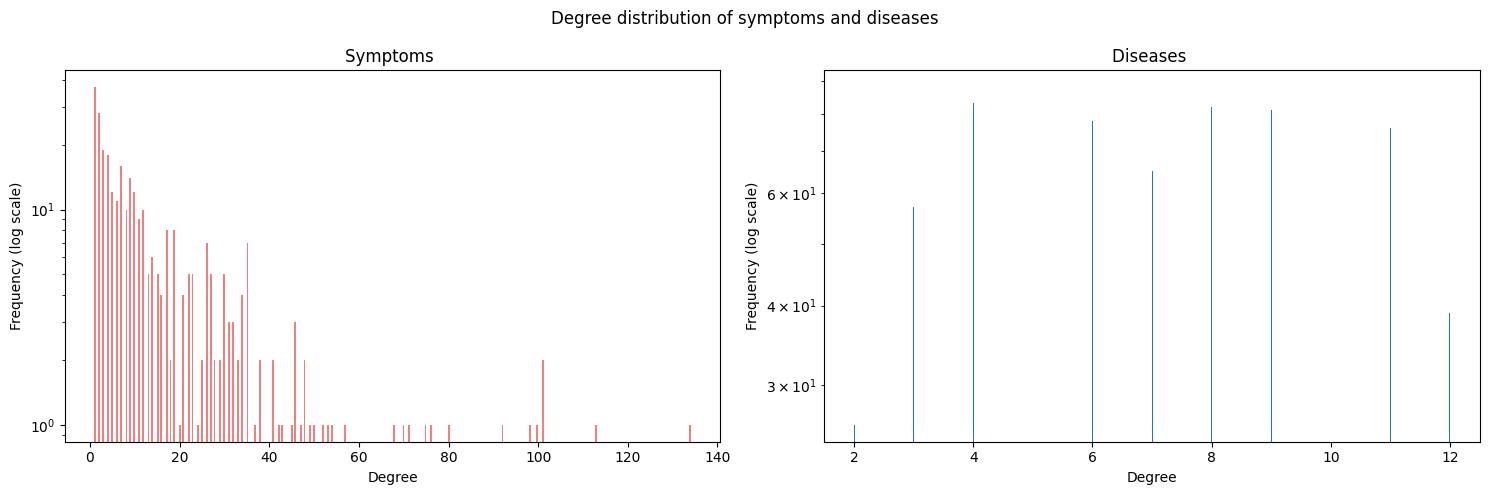
\includegraphics[width=\columnwidth]{degree_distribution.png}
    \caption{Degree Distribution (level 1)}
    \label{fig:DegreeDistribution}
\end{figure}

\subsubsection*{Level-2 Metrics}
Moving to the level-2 metrics, which capture the interconnectedness and broader impact of symptoms or diseases within the network,
we uncovered intriguing patterns (see Figure~\ref{fig:l2_distribution}).
The Symptom Influence (\textit{SI}) at level-2, reflecting the presence of symptoms across diseases and their associations with other symptoms,
exhibited values ranging from 4 to 12.
This suggests that certain symptoms not only co-occur within diseases but also form meaningful connections with a diverse set of other symptoms.
A higher level-2 Symptom Influence (\textit{SI}) implies a symptom's propensity to be associated with a wide range of symptoms,
indicating its potential impact on various disease pathways.\\
On the other hand, the Disease Influence (\textit{DI}) at level-2, quantifying the ripple effects of a disease's symptoms on other diseases,
demonstrated a wider range, typically spanning from 10 to 80.
This broader range signifies that certain diseases have a more extensive influence on the network by affecting a multitude of other diseases.
A higher level-2 Disease Influence (\textit{DI}) implies that a disease's symptoms not only contribute to its immediate associations
but also have far-reaching consequences, affecting a network of interconnected diseases.\\
These results highlight the diverse roles played by symptoms and diseases in influencing the network when considering higher-order interactions.
The observed power-law distribution in level-1 metrics extends to level-2 metrics,
reaffirming the presence of both highly influential and less influential nodes in the network's intricate structure.
The power-law behavior (shown in Figure~\ref{fig:powerlaw_hid_metrics}) suggests that a few symptoms and diseases play central roles in the network,
impacting a wide array of others, while the majority exhibit lower levels of influence.

\begin{figure}[H]
    \centering
    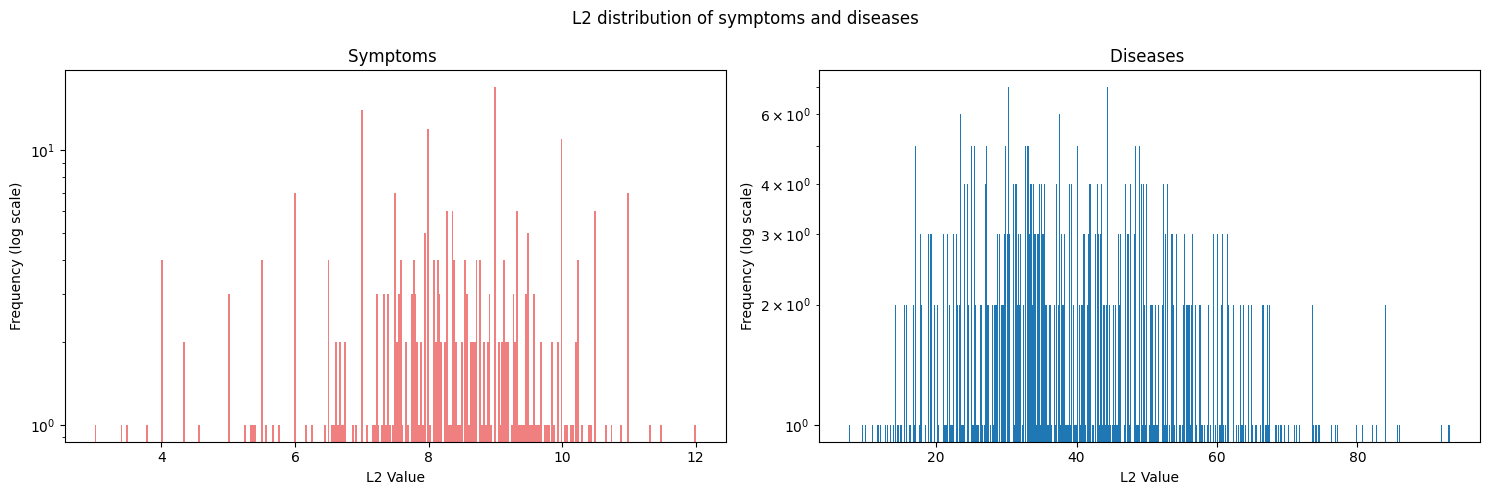
\includegraphics[width=\columnwidth]{L2_distribution.png}
    \caption{L2 Distribution for both symptoms and diseases}
    \label{fig:l2_distribution}
\end{figure}

\begin{figure}[H]
    \centering
    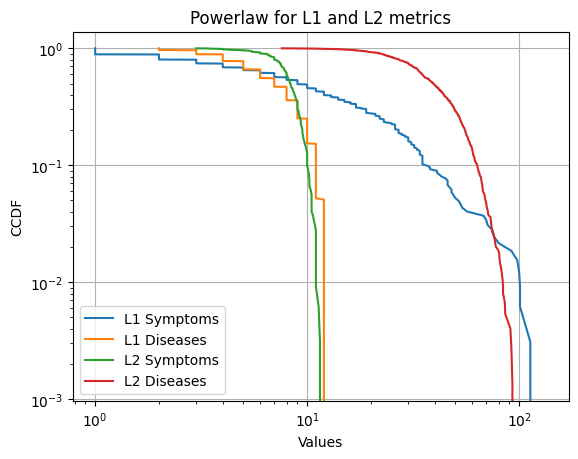
\includegraphics[width=\columnwidth]{powerlaw_hid_metrics.png}
    \caption{Power Law Distribution of the level 1 and level 2 metrics}
    \label{fig:powerlaw_hid_metrics}
\end{figure}
\subsubsection*{Statistical Validation of SI and DI}

In our statistical validation of the Symptom Influence (\textit{SI}) and Disease Influence (\textit{DI}) indices at level-2,
we aimed to discern whether these higher-order metrics provide additional information compared to level-1,
and whether this information is statistically significant.
Our null hypothesis (\textbf{H0}) posited that level-2 metrics do not offer additional insights beyond level-1,
while the alternative hypothesis (\textbf{H1}) suggested the opposite.\\
Upon generating 5000 random networks with the same level-1 properties as the original network,
we calculated z-scores for both Symptom Influence (\textit{SI}) and Disease Influence (\textit{DI}) at level-2.\\
Remarkably, the z-score distribution (Figure~\ref{fig:pdf_z_score}) for both symptoms and diseases exhibited a shape quite similar to a Gaussian distribution,
with means close to zero.\\
For symptoms, the z-scores ranged between -4 and 3, indicating that the level-2 Symptom Influence (\textit{SI})
values were generally lower than the mean but still within a reasonable range. This suggests that, on average,
symptoms tend to exhibit a level-2 influence that aligns closely with the overall network structure.\\
Similarly, for diseases, the z-scores ranged from -3 to 4, signifying that the level-2 Disease Influence
(\textit{DI}) values were distributed around the mean.
This implies that diseases, on average, have a level-2 influence that aligns with the overall network structure,
showcasing a balance between localized effects and broader impacts.\\
The proximity of the mean to zero in both distributions suggests that, on average,
the level-2 metrics for both symptoms and diseases do not significantly deviate from the null model.
However, the broader range of z-scores signifies the presence of nodes with both positive and negative deviations,
underscoring the heterogeneous nature of influences within the symptom-disease network.\\
In conclusion, our statistical validation reinforces that while the level-2 metrics follow a distribution akin to a Gaussian,
the nuanced deviations reflected by the z-scores
for both symptoms and diseases underscore the diverse and context-dependent nature of their influences within the intricate network structure.

\begin{figure}[H]
    \centering
    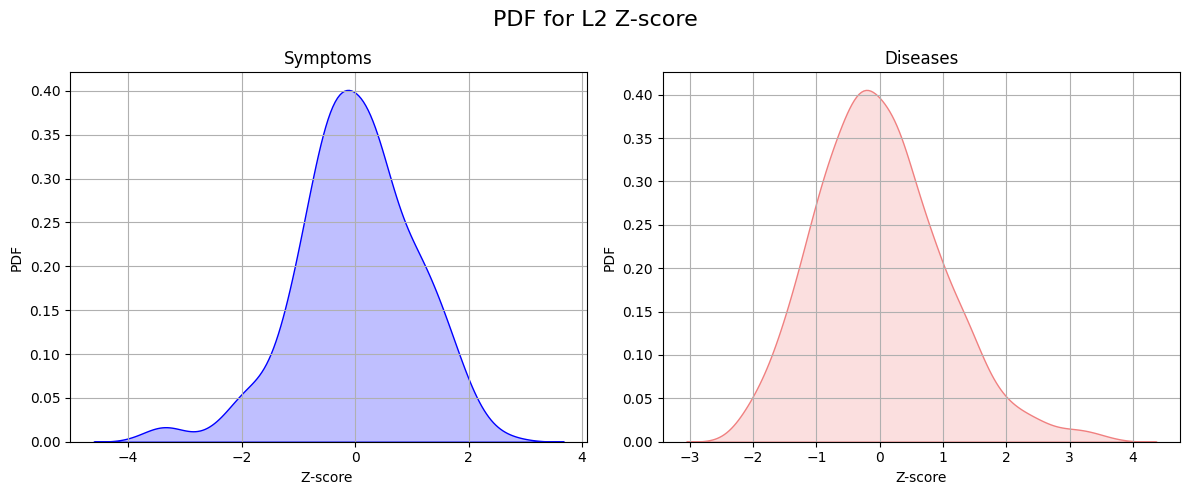
\includegraphics[width=\columnwidth]{PDF_z_score.png}
    \caption{probability density function of the z-score}
    \label{fig:pdf_z_score}
\end{figure}
% END: degree distribution and power law

\subsection{Betweenness Centrality}
% BEGIN: betweenness centrality
The examination of betweenness centrality in our bipartite network, as depicted in Figure~\ref{fig:bet_all},
reveals a Power Law Distribution, indicative of a scale-free structure. This implies the presence of a few central
nodes that act as pivotal connectors, while the majority of nodes exhibit lower betweenness centrality.

\begin{figure}[H]
    \centering
    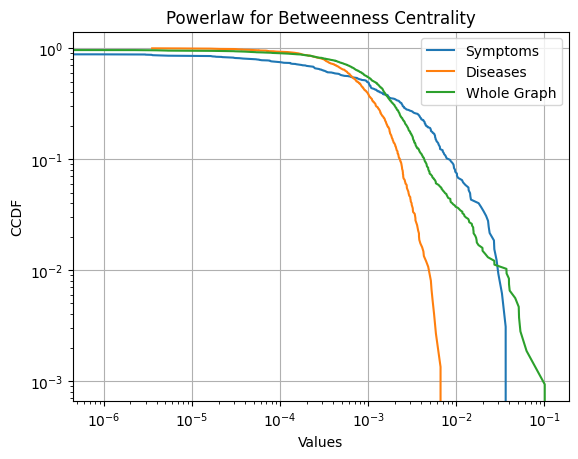
\includegraphics[width=\columnwidth]{bet_all.png}
    \caption{Betweenness Centrality CDFs}
    \label{fig:bet_all}
\end{figure}
\noindent
Upon dissecting the centrality values into symptoms and diseases (see Figures~\ref{fig:bet_diseases} and~\ref{fig:bet_symptoms}),
a notable observation emerges: symptoms tend to have higher betweenness centrality compared to diseases. To decipher the
significance of this result, it's essential to delve into the interpretation of betweenness centrality.

\begin{figure}[H]
    \centering
    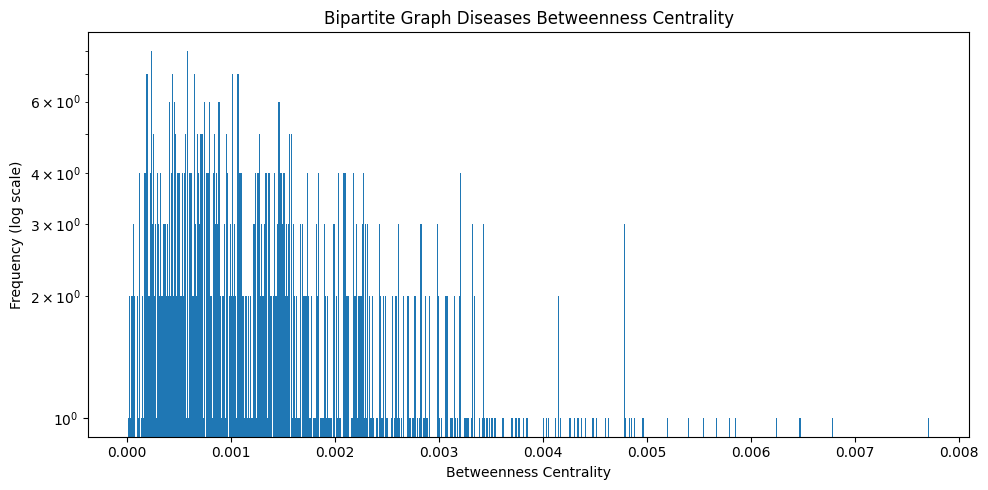
\includegraphics[width=\columnwidth]{bet_diseases.png}
    \caption{Betweenness Centrality of the diseases}
    \label{fig:bet_diseases}
\end{figure}
\noindent
\begin{figure}[H]
    \centering
    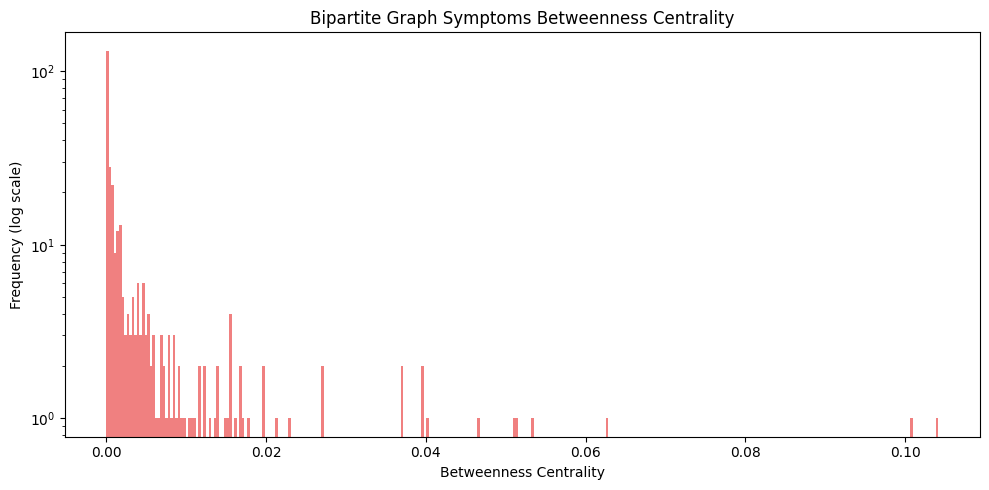
\includegraphics[width=\columnwidth]{bet_symptoms.png}
    \caption{Betweenness Centrality of the symptoms}
    \label{fig:bet_symptoms}
\end{figure}
\noindent
In general, a symptom exhibits high betweenness centrality when it is linked to numerous diseases, and these diseases,
in turn, are connected to a relatively limited set of symptoms. Conversely, a disease attains high betweenness centrality
when it connects to numerous symptoms, and these symptoms are associated with relatively few diseases.\\
Analyzing our results (L1 and L2), it becomes evident that the higher betweenness centrality of symptoms is attributed
to their connections with a multitude of diseases, while diseases, on the contrary, are linked to a relatively limited
number of symptoms. From a predictive standpoint, this outcome presents a challenge as each symptom is not sufficiently
specific, contributing to a broad array of disease classes.\\
Figure~\ref{fig:bet_top} highlights the top 10 nodes with the highest betweenness centrality, all of which are symptoms.
As anticipated, these symptoms are more generic in nature, aligning with their central role in connecting various diseases.

\begin{figure}[H]
    \centering
    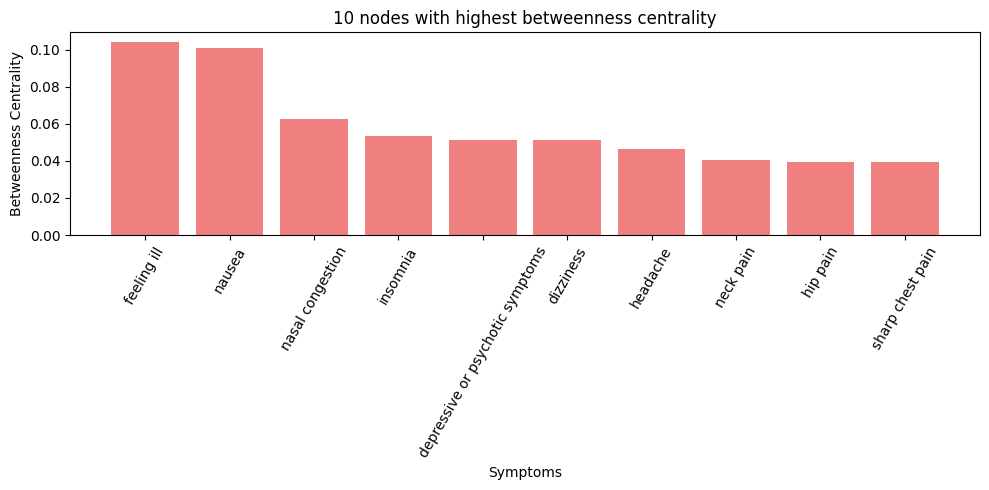
\includegraphics[width=\columnwidth]{bet_top.png}
    \caption{Top 10 nodes with the highest betweenness centrality}
    \label{fig:bet_top}
\end{figure}
\noindent
% END: betweenness centrality

\subsection{Communities}

% BEGIN: communities
The identification of communities within the network serves a dual purpose – facilitating network interpretation
and enhancing the capabilities of our ML prediction model.\\
From a network interpretation perspective, communities offer insights into disease-symptom relationships.
A community of symptoms signifies a set of symptoms that frequently co-occur within the same diseases, while a
community of diseases identifies a set of diseases often co-occurring within the same symptoms. The sizes of
different communities are illustrated in Figure~\ref{fig:com_sizes_all}.

\begin{figure}[H]
    \centering
    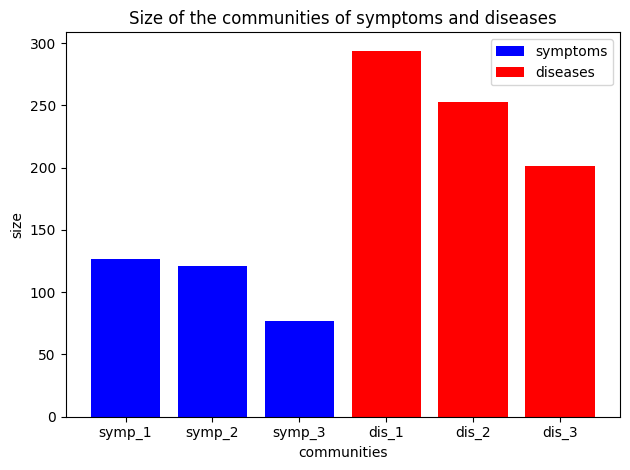
\includegraphics[width=\columnwidth]{com_sizes_all.png}
    \caption{Sizes of the communities of symptoms and diseases}
    \label{fig:com_sizes_all}
\end{figure}
\noindent
For clinical relevance, examining symptoms communities provides valuable information about diseases associated
with these symptoms. This is exemplified in Figures~\ref{fig:com1_symptoms},~\ref{fig:com2_symptoms},
and~\ref{fig:com3_symptoms}. As an illustration, in the community 1 of symptoms (Figure~\ref{fig:com1_symptoms}),
`herniated disk' is the third most pointed disease by the symptoms of the community, with each symptom pointing,
on average, to three diseases.

\begin{figure}[H]
    \centering
    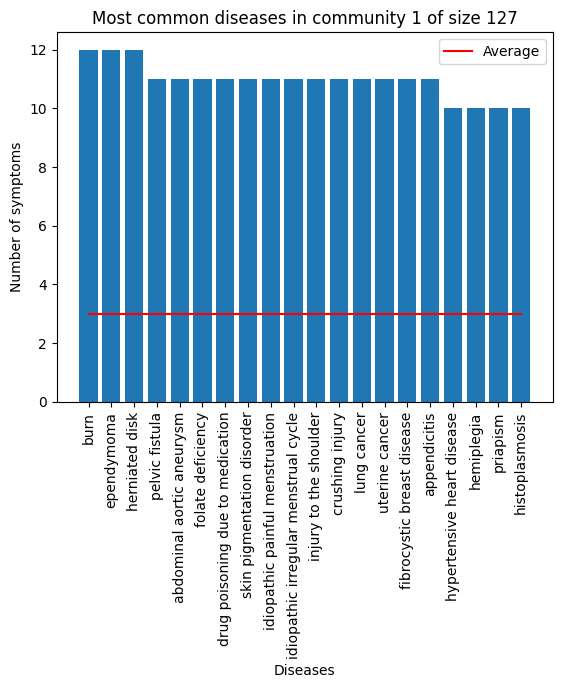
\includegraphics[width=\columnwidth]{com1_symptoms.png}
    \caption{Community 1 of symptoms}
    \label{fig:com1_symptoms}
\end{figure}
\noindent
A similar study can be conducted for communities of diseases, as depicted in Figures~\ref{fig:com1_diseases},
~\ref{fig:com2_diseases},~\ref{fig:com3_diseases}. This information aids in profiling diseases and understanding
the significance of each symptom. For instance, in community 1 of diseases (Figure~\ref{fig:com1_diseases}),
the symptom `sharp abdominal pain' is present in almost half of the diseases in the community, indicating its
generic nature and limited discriminatory value.

\begin{figure}[H]
    \centering
    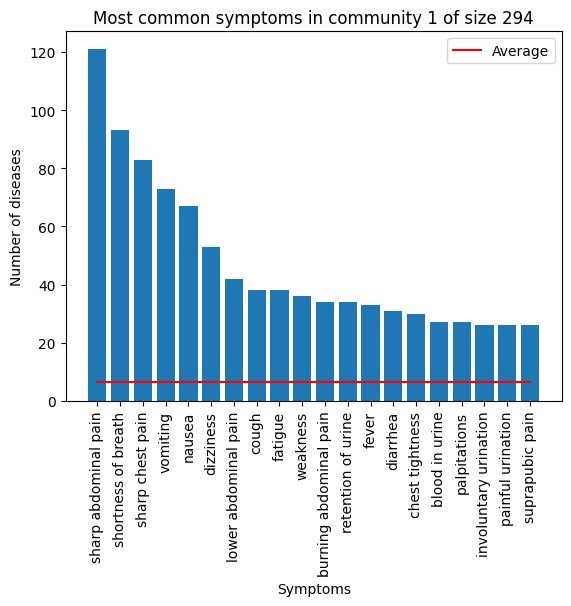
\includegraphics[width=\columnwidth]{com1_diseases.png}
    \caption{Community 1 of diseases}
    \label{fig:com1_diseases}
\end{figure}
\noindent
Transitioning to the creation of features for the ML model, two types of features were developed:\\

\begin{itemize}
    \setlength\itemsep{1em} % set space between items

    \item \textbf{Community Count:} This feature counts how many symptoms of the symptom vector belong to each community.
          Each symptom community is characterized by different pointed diseases. The model can learn to prioritize
          diseases associated with the community with the highest count.

    \item \textbf{Community Size:} This feature replaces each symptom in the symptom vector with the size of the
          community to which the symptom belongs. It enables the model to distinguish between symptoms belonging to small and
          large communities, injecting community information into the model beyond basic one-hot encoding of symptoms.
\end{itemize}
\noindent
\vspace{0.4cm}
It is noteworthy that communities can also contribute to improving the computational efficiency of the model.
For example, a symptom associated with many diseases may be less informative and could potentially be removed from the
symptom vector. However, we opted for a comprehensive approach using a combination of L1 and L2 measures to address this issue.

% END: communities

\subsection{Most Important Actors}
\label{subsec:most_important_actors}
% BEGIN: most important symptoms/diseases (4 classes)

As previously mentioned, our objective extends beyond feature extraction; we aim to leverage network information to
enhance the computational efficiency of the model. The strategy involves reducing the number of symptoms,
retaining only the most significant ones, to decrease training time while maintaining high accuracy.
Various approaches were tested, including L1, L2, betweenness centrality, and the degree of the unipartite projection
of symptoms. To select the most appropriate approach, we examined the correlation between these features
(Figure~\ref{fig:feat_corr}). Indeed, a high correlation between features means that they provide
similar information, and therefore retaining both features would be redundant. On the other hand,
a low correlation between features indicates that they provide complementary information, and this enhances
in a considerable way the quality of the choice.\\
For this reason, as clearly shown in Figure~\ref{fig:feat_corr}, we decided to use L1 and L2 to discriminate
among the symptoms in a more effective manner.

\begin{figure*}[!t]
    \centering
    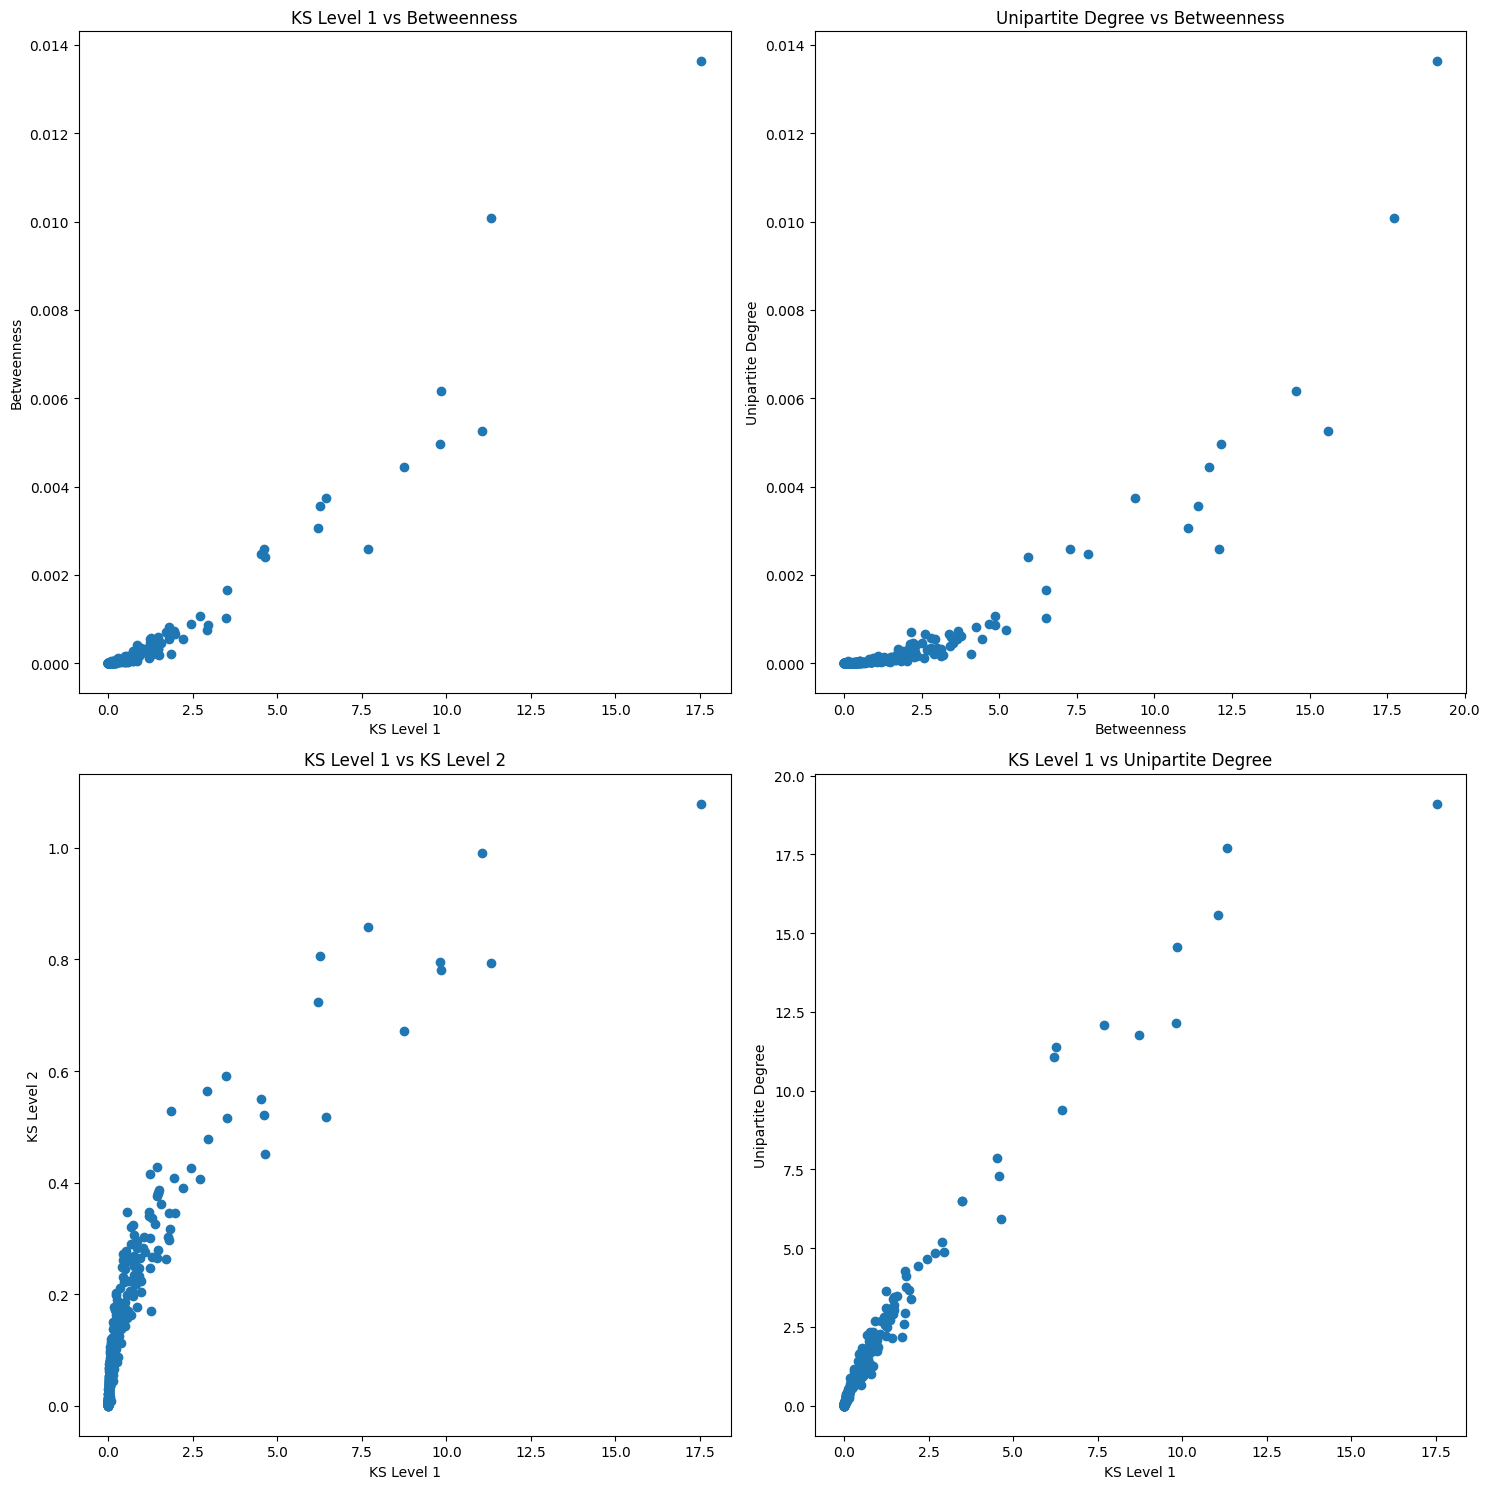
\includegraphics[width=\textwidth]{feat_corr.png}
    \caption{Correlation between features}
    \label{fig:feat_corr}
\end{figure*}

\noindent
While the analytical approach relying on correlation analysis lays a robust foundation for feature selection,
it is equally crucial to invest effort in interpreting the results. This interpretive step facilitates a
more profound understanding of the solution.

To shed light on these classes, a brief reminder of the meanings of L1 and L2 is warranted. L1 denotes the number
of diseases associated with a symptom, whereas L2 quantifies the number of symptoms linked to those diseases.
As a result, we categorize the features into the following classes:\\

\begin{itemize}
    \setlength\itemsep{1em}
    \item \textbf{High L1 - High L2}: Symptoms with high degree and high L2. These symptoms are less crucial for
          prediction as they contribute to many classes (diseases), which are also connected to many other symptoms.
    \item \textbf{High L1 - Low L2}: Symptoms with high degree and low L2. These symptoms should not be removed a
          priori since they can be useful. For instance, a symptom may be associated with many diseases, but those
          diseases may only be associated with that symptom. In this case, the symptom is very important for prediction.
    \item \textbf{Low L1 - High L2}: Symptoms with low degree and high L2. These symptoms may be important for
          prediction, as they contribute to few diseases.
    \item \textbf{Low L1 - Low L2}: Symptoms with low degree and low L2. These symptoms are the most important
          for prediction since they contribute to few classes (diseases), and those classes are also connected to
          few other symptoms.
\end{itemize}
\vspace{0.4cm}

\noindent
According to the above considerations, we can start from the last class and iteratively add symptoms from the
other classes, monitoring the impact on both accuracy and training time.
The results are analyzed in Section~\ref{sec:results_ML}.\\

To practically create the classes, we need to define thresholds for L1 and L2. We decided to consider
a symptom as very important for our model if it is present in less than 0.5 times the average of L1 diseases,
translating into a threshold of 8.21 for L1. Consequently, we adjusted the L2 threshold to maintain a proper balance
between the classes, setting it to 8.

Figures~\ref{fig:symptoms_classes} and~\ref{fig:l1_l2_division} illustrate the division of symptoms into the four classes.
The same analysis was conducted for diseases, in this case focusing on the high-L1-high-L2 class, which contains
the most complex diseases under a symptomatology perspective. The results are reported in Figures~\ref{fig:diseases_classes}
and~\ref{fig:high_l1_high_l2_class}.\\


\begin{figure}[H]
    \centering
    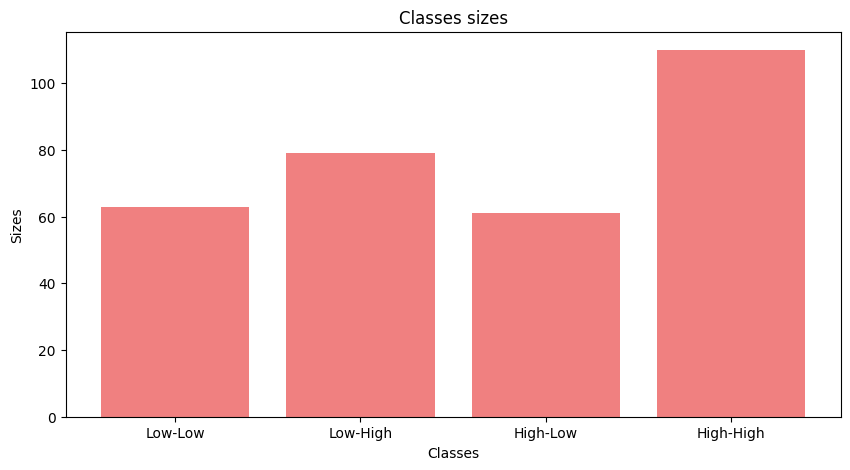
\includegraphics[width=\columnwidth]{symptoms_classes.png}
    \caption{Symptoms divided into the four classes}
    \label{fig:symptoms_classes}
\end{figure}

\begin{figure}[H]
    \centering
    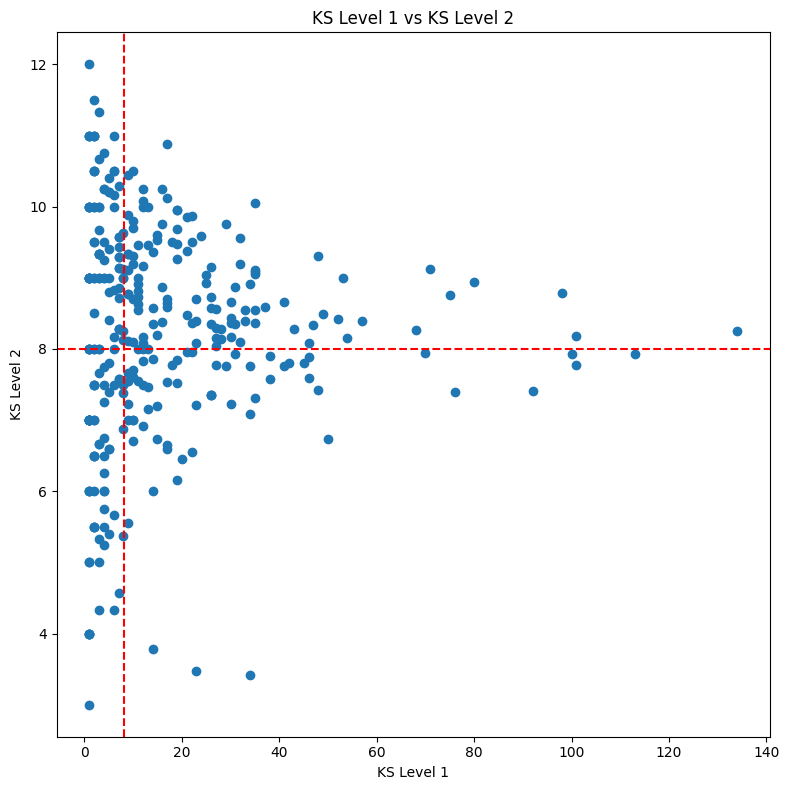
\includegraphics[width=\columnwidth]{l1_l2_division.png}
    \caption{Division based on L1 and L2 values}
    \label{fig:l1_l2_division}
\end{figure}
\noindent

\noindent
To provide a complete picture of the most important symptoms we report the composition of the low-L1-low-L2 class
in Figure~\ref{fig:low_l1_low_l2_class}.\\

\begin{figure*}[!t]
    \centering
    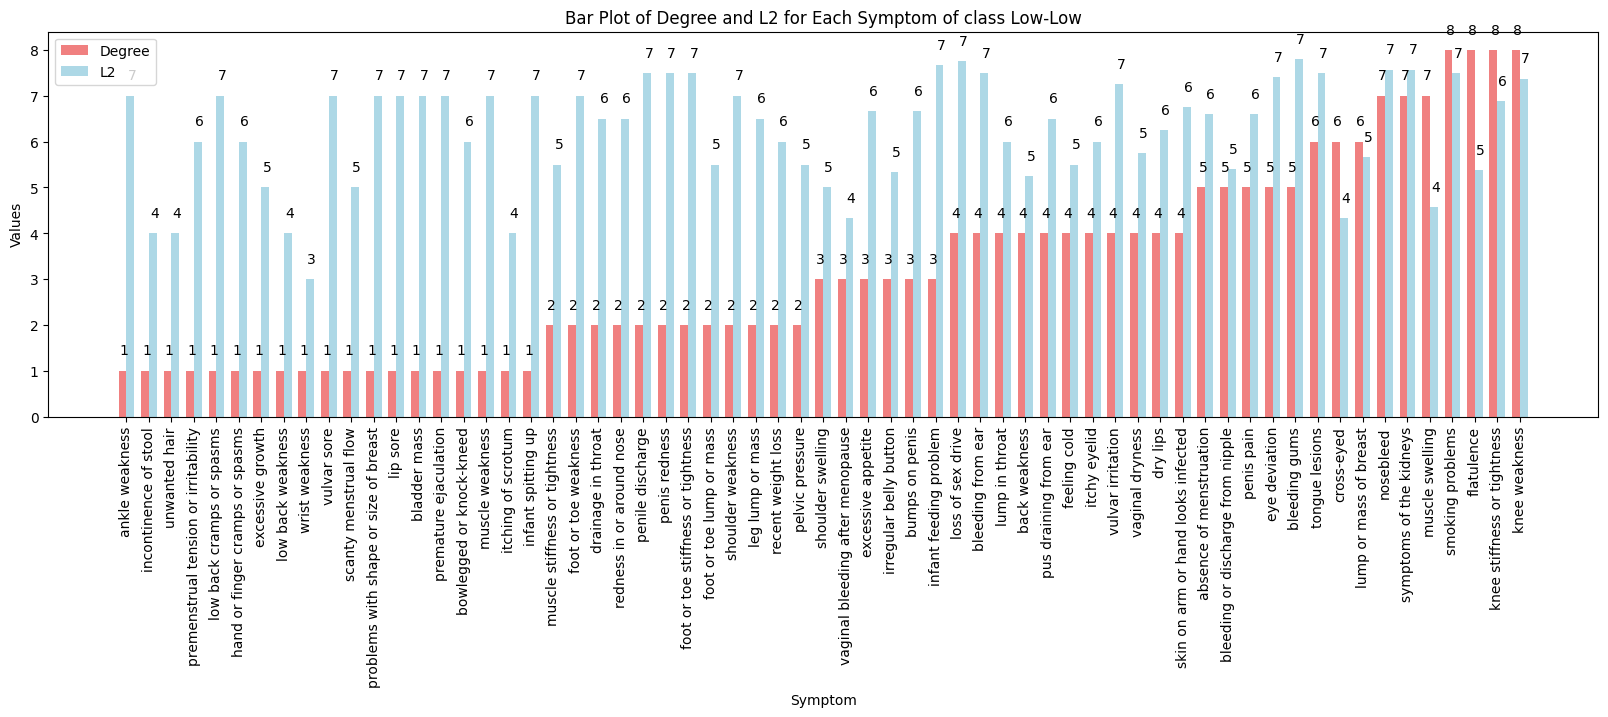
\includegraphics[width=\textwidth]{low_l1_low_l2_class.png}
    \caption{Composition of the low-L1-low-L2 class for symptoms}
    \label{fig:low_l1_low_l2_class}
\end{figure*}

% END: most important symptoms/diseases (4 classes)






% - degree distribution and power law
% - most important symptoms/diseases (4 classes) 
% - communities
% - L2 has no sense, it's right that z-score low value
% - Meaning of Z-score
% - betweenness centrality
% - clustering coefficient

% ------------------- Methodology and Results ML -------------------

% How we built the ML model 
\section{ML Model Methodology}
This section provides a comprehensive overview of the methodologies employed in the construction of the machine 
learning model. The discussion encompasses various techniques designed to handle the intricacies of model building, 
coupled with a logical flow that guides the entire process.

% ------------------- Data Preparation -------------------

\subsection{Data Balancing}
% - Face the unbalanced dataset problem



% ------------------- Feature Extraction -------------------

\subsection{Feature Extraction}
% - Prepare the features and normalization
A pivotal phase in constructing a machine learning model is feature extraction. In addition to the one-hot vector representation 
of symptoms, the network analysis affords us the following features:

\begin{itemize}
    \setlength\itemsep{0.4em} % set space between items
    \item \textbf{L1 and L2 Measures}: A vector with values representing the L1 and L2 measures for each symptom.
    \item \textbf{Betweenness Centrality}: A vector with values denoting the betweenness centrality of each symptom.
    \item \textbf{Community Count}: A vector indicating the number of symptoms belonging to each community.
    \item \textbf{Community Size}: A vector replacing symptoms with the size of the community to which they belong.
\end{itemize}
\vspace{0.4cm}

Given the diverse scales of these features, normalization becomes imperative for their cohesive integration into the model 
without introducing biases. To achieve this, we opted for \textit{MaxAbs} normalization. This normalization scales each feature 
individually, ensuring that the maximal absolute value of each feature in the training set becomes 1.0, while preserving the sparsity of data.


% ------------------- Operative Flow -------------------

\subsection{Operative Flow}
% - Operative Flow
	% - select best parameters for symptoms one hot only
	% - select best parameters for combination of other features (best combination is chosen with random parameters looking at the accuracy)
	% - train for each model the two version above with optimal parameters
	% - pick the best model according to accuracy
	% - train the best model with whole dataset and reduce the number of features

Once the features are ready, the core part of the model-building process can begin. 
We trained three different models: a Logistic Regression, a Random Forest, and a Multi-Layer Perceptron (MLP).

For each model, we faced the challenge of selecting both the best parameters and the most effective features. 
The interdependence between these two aspects makes the optimal approach to explore all the possible combination of features
and for each combination trying all the parameters combination. This approach is not feasible in terms of computational effort
leading us to adopt a greedy approach. We firstly split the features into two 
groups: the symptoms' one-hot vector and the remaining features. The former is used to train a base model, 
while the latter is utilized to explore the potential improvement brought by the new features.

Using Algorithm \ref{alg:feature_selection}, we determined the best feature combination for each group (symptoms and other features).
Subsequently, given the optimal feature combination, we identified the best parameter combination using Algorithm 
\ref{alg:best_selection}. Each model was then trained with the best parameters and the best features combination, 
and the model with the highest accuracy was chosen. Finally, the best overall model was trained with the entire dataset.


\begin{algorithm}[H] \small
	\caption{Feature Selection Algorithm}\label{alg:feature_selection}
	
	\begin{algorithmic}[1]
	
	\State BestFeatureComb $\gets$ EmptySet
	
	\For{each model}
	    \State CurrentModel $\gets$ EmptyModel
	    \State BestModAccuracy $\gets$ 0
	    \State Parameters $\gets$ InitializeRandomParameters
	
	    \For{i = 1 to NumberOfFeatures}
	    		\State BestAccuracy $\gets$ -1

			\For{each feature}
				\State TrainModel(CurrentModel, Parameters)
			
				\State CurrentAccuracy $\gets$ GetAccuracy(CurrentModel)
			
				\If{CurrentAccuracy $>=$ BestAccuracy}
					\State BestAccuracy $\gets$ CurrentAccuracy
					\State BestFeature $\gets$ feature
					
				\EndIf
				\State UpdateModel(CurrentModel, BestFeature)
			\EndFor
			\State FreezeFeatures(CurrentModel)
			\State ModelAccuracy[i] $\gets$ GetAccuracy(CurrentModel)
			\State FeaturesComb[i] $\gets$ GetFeat(CurrentModel)
	
	    \EndFor
	
	    \State BestComb $\gets$ FeaturesComb[Max(ModelAccuracy)]
	    \State BestFeatureComb $\gets$ BestComb $\cup$ BestFeatureComb
	
	\EndFor
	
	\State \textbf{return} BestFeatureComb
	\end{algorithmic}
\end{algorithm}

\begin{algorithm}[H] \small
	\caption{Best Model Selection Algorithm}\label{alg:best_selection}
	
	\begin{algorithmic}[1]
	
	\State CurrentAccuracy $\gets$ 0
	\For{each model}
	    
	    \State CreateGrid(Parameters)
	    \State BestParameters $\gets$ GridSearchCV(model)
	    \State TrainModel(model, BestParameters)
	    \State CurrentAccuracy $\gets$ GetAccuracy(model)

	    \If{CurrentAccuracy $>=$ BestAccuracy}
			\State BestAccuracy $\gets$ CurrentAccuracy
			\State BestModel $\gets$ model
			\State BestParameters $\gets$ Parameters
	    \EndIf

	\EndFor

	\State FullDataTrain(BestModel, BestParameters)
	\State BestAccuracy $\gets$ GetAccuracy(BestModel)
	\State ReduceFeatures(BestModel, BestParameters)
	
	\State \textbf{return} BestParameters, BestModel, BestAccuracy
	\end{algorithmic}
\end{algorithm}


At the conclusion of these procedures, we obtained the following two models:\\

\begin{itemize}
    \setlength\itemsep{0.4em} % set space between items
    \item \textbf{Symptoms Model}: The best model with the optimal parameters and the symptoms as features
    \item \textbf{Other Features Model}: The best model with the optimal parameters and the best features combination
\end{itemize}
\vspace{0.4cm}

With these models in hand, we could compare their prediction performance to evaluate whether the network 
features contributed to an accuracy improvement. Additionally, we applied the feature reduction technique discussed 
in Section \ref{sec:feature_reduction} to both models, assessing whether network features could reduce computational 
complexity without compromising accuracy.


% - Face the unbalanced dataset problem
% - select best parameters for symptoms one hot only
% - select best parameters for combination of other features (best combination is chosen with random parameters looking at the accuracy)
% - Face the problem of normalization
% - train for each model the two version above with optimal parameters
% - pick the best model according to accuracy

% Results of the ML model (plots and tables)
\section{ML Model Results}\label{sec:results_ML}
In this section we present the results of the ML models we have trained. We then deeply inspect the best performing model,
in order to understand its features and its performance.


% --------------- Model Selection ---------------

\subsection{Model Selection}\label{subsec:results_ML_model_selection}
As previously shown by the operative flow in Figure~\ref{fig:ML_operative_flow}, there are several phases involved in the
selection of the optimal prediction model. Given our limited resources we chose to take a greedy approach by performing
the feature selection first, and then optimizing the hyperparameters at a later time for each of the three models considered.
% MATTEO
% - Matrix plot of stepwise (which is results of algorithm 1) for each model --> to justify the chosen features
\subsubsection*{Features Selection}
To reduce the amount of time spent training the models to select the best hyperparameters, it is best to first limit the
number of features considered. The selection of the most useful features was performed using a forward stepwise selection,
following a greedy a approach that aims at maximizing the accuracy. The hyperparameters were initalized with the default
values provided by the library scikit-learn.\\
As depicted in Figure~\ref{fig:stepwise_acc_logreg}, we can see that the best accuracy with the logistic regression
model is reached after the third iteration, with little improvement with respect to the model using a single feature.
This kind of model seems to favor information about communities and centrality, while the L1 and L2 measures in some cases actually worsen its performance.
\begin{figure}[H]
	\centering
	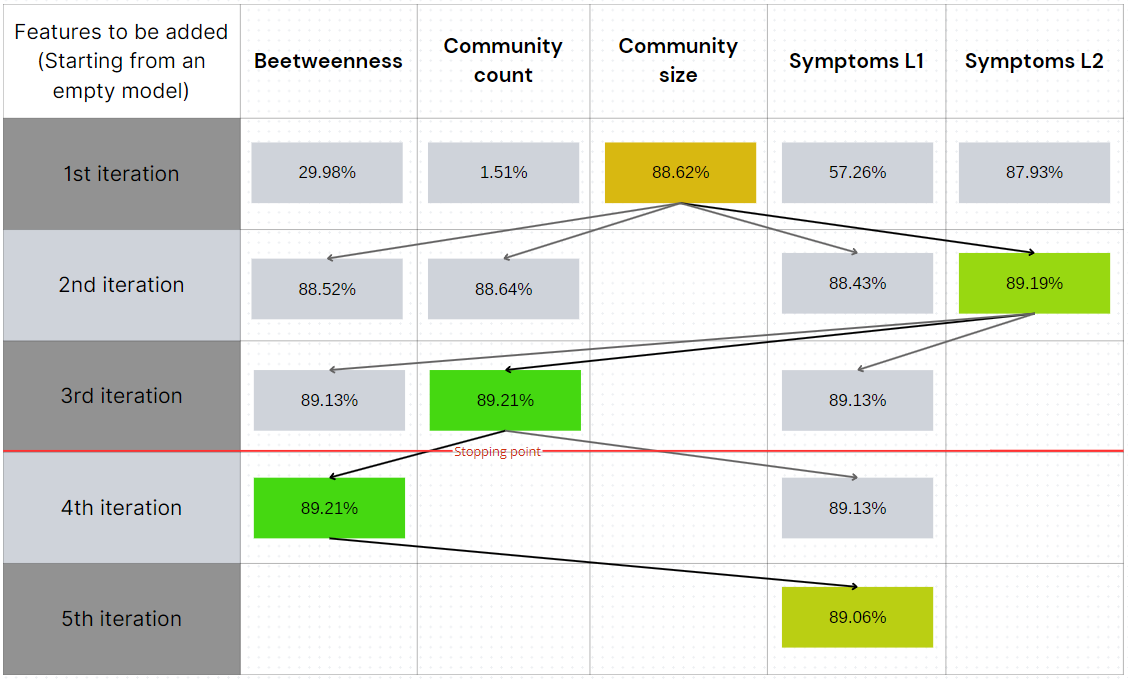
\includegraphics[width=\columnwidth]{stepwise_acc_logreg.png}
	\caption{Accuracy of the logistic regression models over the iterations of the forward stepwise feature selection}\label{fig:stepwise_acc_logreg}
\end{figure}
\noindent
Figure~\ref{fig:stepwise_acc_randomforest} shows that the random forest models behave similarly to the logistic regression,
as the best accuracy is reached after the same number of steps, employing the same features.
These results start to reveal which features are the best when it comes to classification.
It is also worth noting that the best random forest model has a slightly worse accuracy than logistic regression,
but that might be due to the random choice of the model's parameters.

\begin{figure}[H]
	\centering
	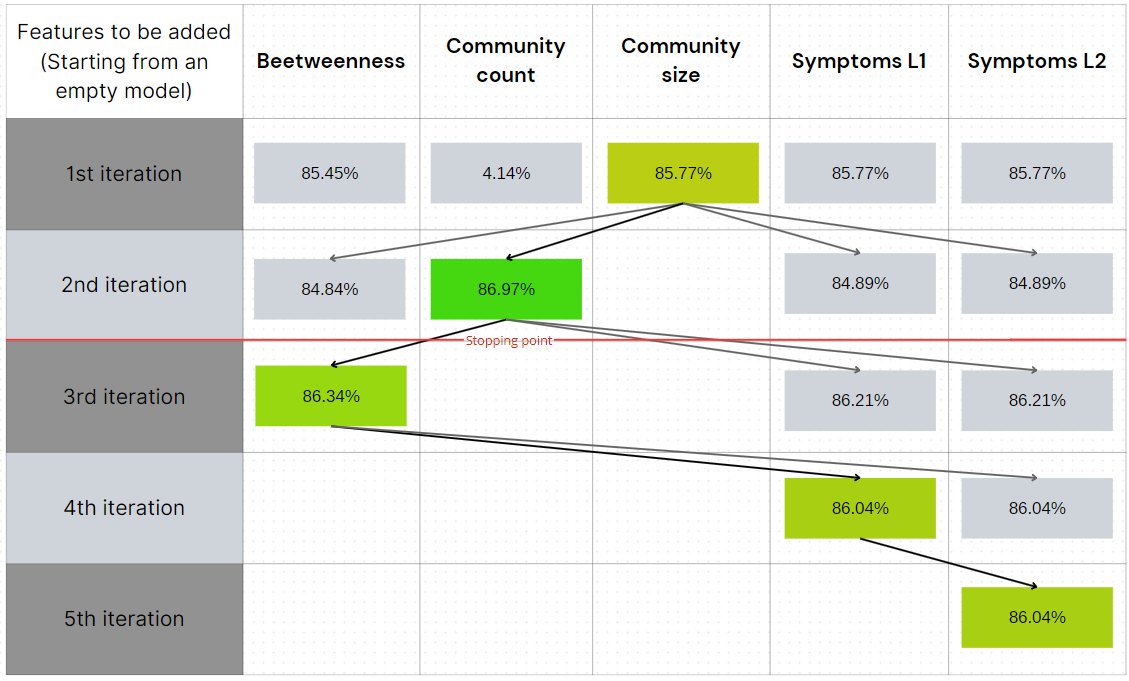
\includegraphics[width=\columnwidth]{stepwise_acc_randomforest.png}
	\caption{Accuracy of the random forest models over the iterations of the stepwise feature selection}\label{fig:stepwise_acc_randomforest}
\end{figure}
\noindent
The multi-layer perceptron model exhibits a different performance from the other two,
given by the fact that the accuracy starts to lower after adding the second feature.
As underlined by Figure~\ref{fig:stepwise_acc_mlp}, with respect to the other models information about the betweenness
is not needed to achieve the best possible results, which could be explained by the better ability of the MLP to adapt to non-linearities.
This particular implementation of neural network has one hidden layer with 100 neurons, and in our case its performance is better
than the random forest model, but still slightly worse than the logistic regression. We expect this to change after the optimization of the hyperparameters.

\begin{figure}[H]
	\centering
	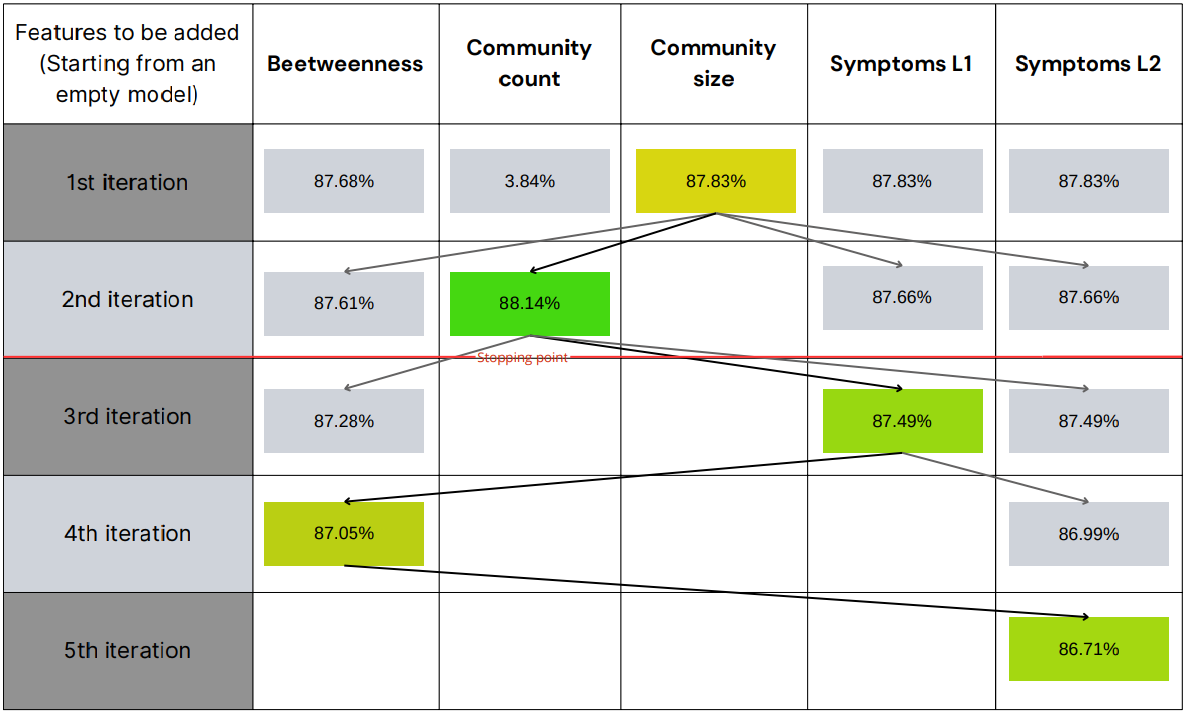
\includegraphics[width=\columnwidth]{stepwise_acc_mlp.png}
	\caption{Accuracy of the MLP models over the iterations of the stepwise feature selection}\label{fig:stepwise_acc_mlp}
\end{figure}


% CRISTIAN
% - Comparison for each model of the selected parameters --> to justify the chosen parameters
\subsubsection*{Hyperparameters Selection}


% ANDREA
% - Comparison of the three models with best combination of features and best parameters
% - precision, recall, AUC, accuracy
\subsubsection*{Model Comparison}\label{subsubsec:results_ML_model_comparison}

As illustrated in Figure~\ref{fig:ML_operative_flow}, our model ensemble now comprises six variants:
three leveraging only symptoms and three incorporating new network-based features. The selection of
the best-performing model from each group was based on test accuracy assessment, where the test is the same balanced dataset
in all cases. Figure~\ref{fig:acc_symptoms}
illustrates consistently low overfitting across all models, showcasing the stability of the symptom-only
models. In contrast, Figure~\ref{fig:acc_new_features}, portraying the accuracy of models with the new
features, reveals some overfitting, particularly in the MLP and Random Forest.\\
The observed tendency for models with new features to exhibit more pronounced overfitting is unsurprising,
given the greater number and complexity of these features compared to symptoms. Notably, despite their different
complexity, all models demonstrate similar test accuracy levels, suggesting that a linear separation
boundary suffices for effective feature classification. Considering this, we retain the Logistic Regression
model as the best-performing model in each group, striking a balance between performance and complexity.

\begin{figure}[H]
	\centering
	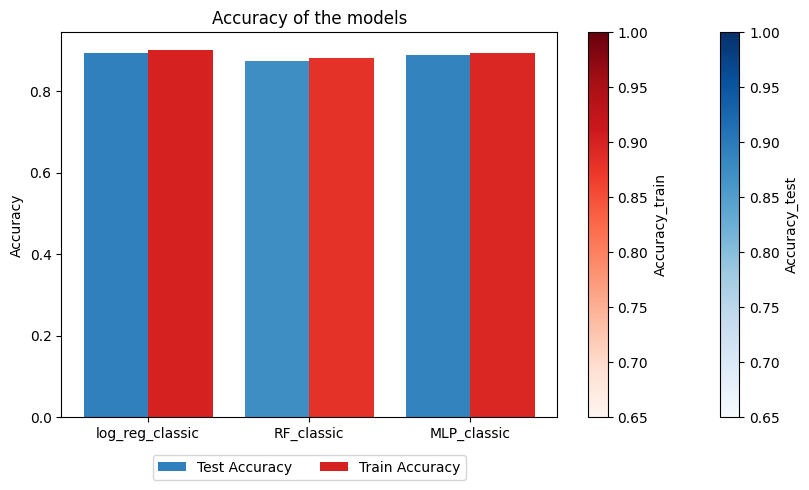
\includegraphics[width=\columnwidth]{acc_symptoms.png}
	\caption{Accuracy of the three models with only symptoms}\label{fig:acc_symptoms}
\end{figure}

\begin{figure}[H]
	\centering
	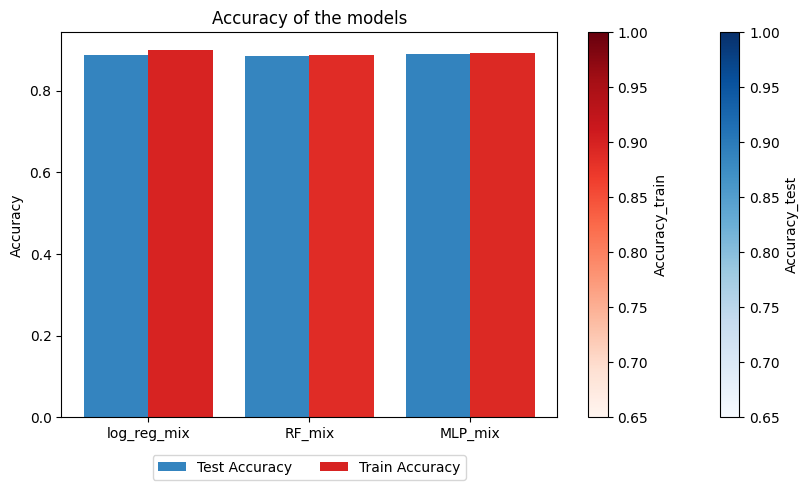
\includegraphics[width=\columnwidth]{acc_new_features.png}
	\caption{Accuracy of the three models with new features}\label{fig:acc_new_features}
\end{figure}



% --------------- New Features Effect ---------------

\subsection{New Features Effect}
% ANDREA
% - compare the best symptoms one hot model with the best one with the new features

\noindent
The best model from each group was further trained on the full balanced dataset to ensure a more reliable
performance evaluation. The results in Figure~\ref{fig:acc_best_models} reveal a minimal difference between
the two groups. This addresses our \textbf{first goal}: the new features, while not improving the model,
offer a comparable performance to using symptoms alone. However, It's essential to note that the new features are
more numerous than the symptoms, contributing to a more complex model. In conclusion, the extracted network
features are not a superior alternative to symptoms.

It is worth to underline that the `simplicity' of the dataset, which leads to a very high accuracy in all models, may also affect the performance
evaluation of the new features, which have a small room to improve the model. Therefore, a possible avenue
for future exploration could involve the use of more complex dataset, to better assess the performance of the
new features.

Another viable option for future work is to use the new features as a complement to the symptoms.


% THE FIGURE IS THE FIGURE OF MODEL FULLY TRAINED ON THE BALANCED DATASET


\begin{figure}[H]
	\centering
	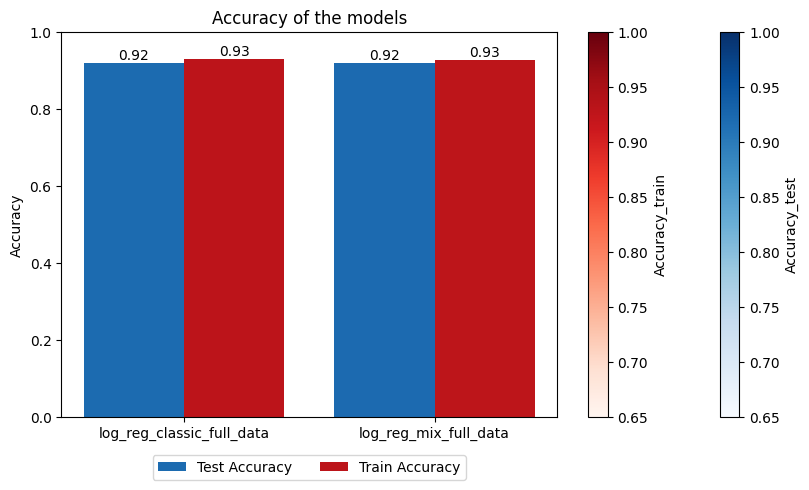
\includegraphics[width=\columnwidth]{acc_best_models.png}
	\caption{Accuracy of the best models from both groups}\label{fig:acc_best_models}
\end{figure}



% --------------- Best Model Performance ---------------

\subsection{Best Model Analysis}
% DAVIDE
% - what are its features
% - confusion matrix computed on the 4 class diseases (HighL1 - HighL2, LowL1 - HighL2, ...)
% - Worst error
% - Most impactful symptoms
\subsubsection*{Performance analysis}
\begin{figure}[H]
	\centering
	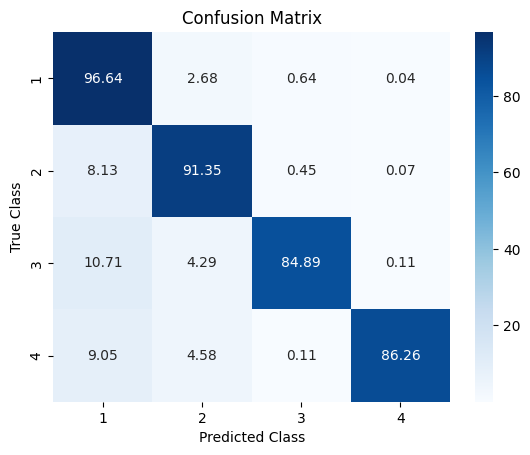
\includegraphics[width=\columnwidth]{conf_matrix_best _model.png}
	\caption{Confusion matrix of the disease classes}\label{fig:conf_matrix}
\end{figure}
\noindent

\begin{figure}[H]
	\centering
	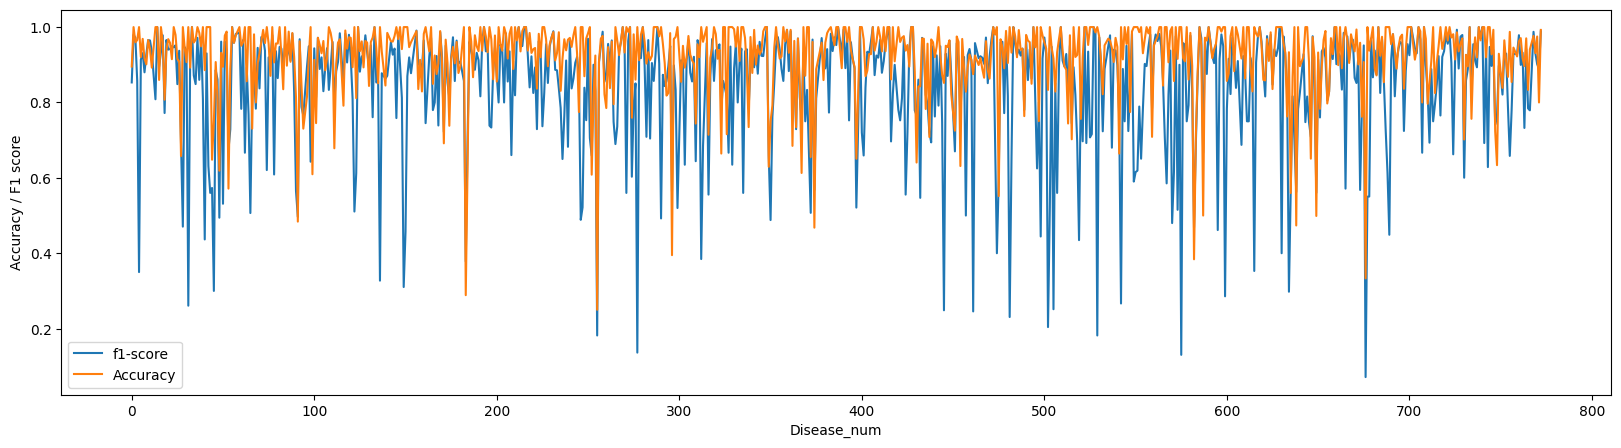
\includegraphics[width=\columnwidth]{accuraci_diseases_best_model.png}
	\caption{Accuracy and f1 score}\label{fig:acc_diseases}
\end{figure}
\noindent


\rowcolors{2}{green!8}{green!18}
\begin{table}[H]
	\centering
	\small
	\begin{tabular}{|c|c|c|}
		\hline
		\textbf{Disease}                    & \textbf{Accuracy} & \textbf{f1-score} \\
		\hline
		mitral valve disease                & 1.0               & 1.000000          \\
		syndrome of inappropriate secretion & 1.0               & 1.000000          \\
		acute bronchospasm                  & 1.0               & 1.000000          \\
		eye alignment disorder              & 1.0               & 1.000000          \\
		reactive arthritis                  & 1.0               & 1.000000          \\
		joint effusion                      & 1.0               & 0.985507          \\
		anal fistula                        & 1.0               & 0.823529          \\
		open wound of the shoulder          & 1.0               & 0.791667          \\
		alzheimer disease                   & 1.0               & 0.769231          \\
		infectious gastroenteritis          & 1.0               & 0.666667          \\
		\hline
	\end{tabular}
	\caption{Accuracy and f1 score for the 10 diseases with the highest accuracy}
	\label{best}
\end{table}


\rowcolors{2}{red!8}{red!18}
\begin{table}[H]
	\centering
	\small
	\begin{tabular}{|c|c|c|}
		\hline
		\textbf{Disease}                     & \textbf{Accuracy} & \textbf{f1-score} \\
		\hline
		premature ventricular contractions   & 0.500000          & 0.666667          \\
		histoplasmosis                       & 0.498876          & 0.560252          \\
		hemiplegia                           & 0.483908          & 0.496462          \\
		acute bronchiolitis                  & 0.473684          & 0.562500          \\
		poisoning due to antimicrobial drugs & 0.467849          & 0.567968          \\
		open wound of the mouth              & 0.394890          & 0.564315          \\
		acute otitis media                   & 0.383938          & 0.468456          \\
		vitamin b12 deficiency               & 0.333333          & 0.071429          \\
		bladder cancer                       & 0.288740          & 0.378102          \\
		otitis media                         & 0.250000          & 0.181818          \\
		\hline
	\end{tabular}
	\caption{Accuracy and f1 score for the 10 diseases with the lowest accuracy}
	\label{worst}
\end{table}

\subsubsection*{Analysis of bladder cancer}

\begin{figure}[H]
	\centering
	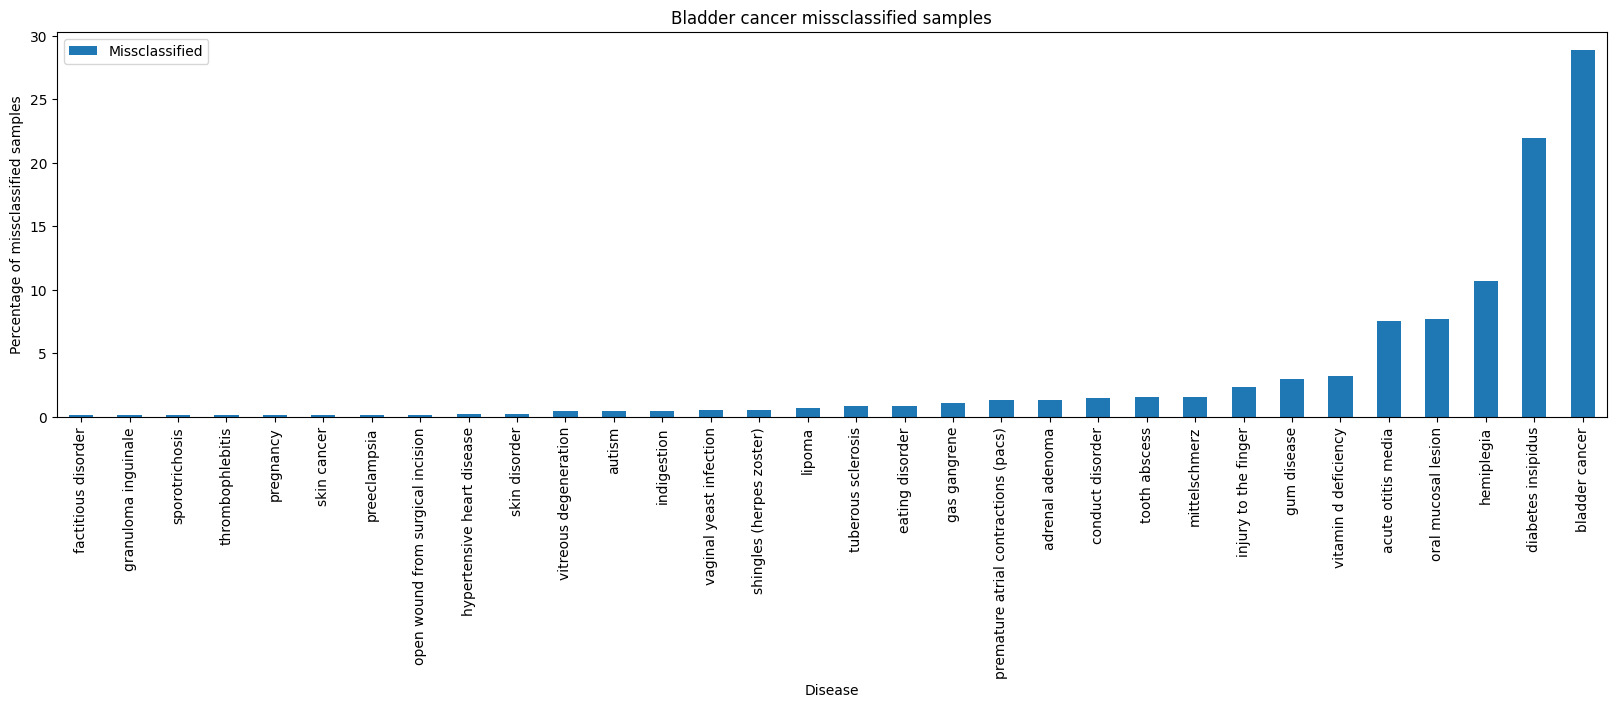
\includegraphics[width=\columnwidth]{bladder_cancer_missclassified.png}
	\caption{Percentage of bladder cancer samples misclassified}\label{fig:cancer_missclassified}
\end{figure}
\noindent

\begin{figure}[H]
	\centering
	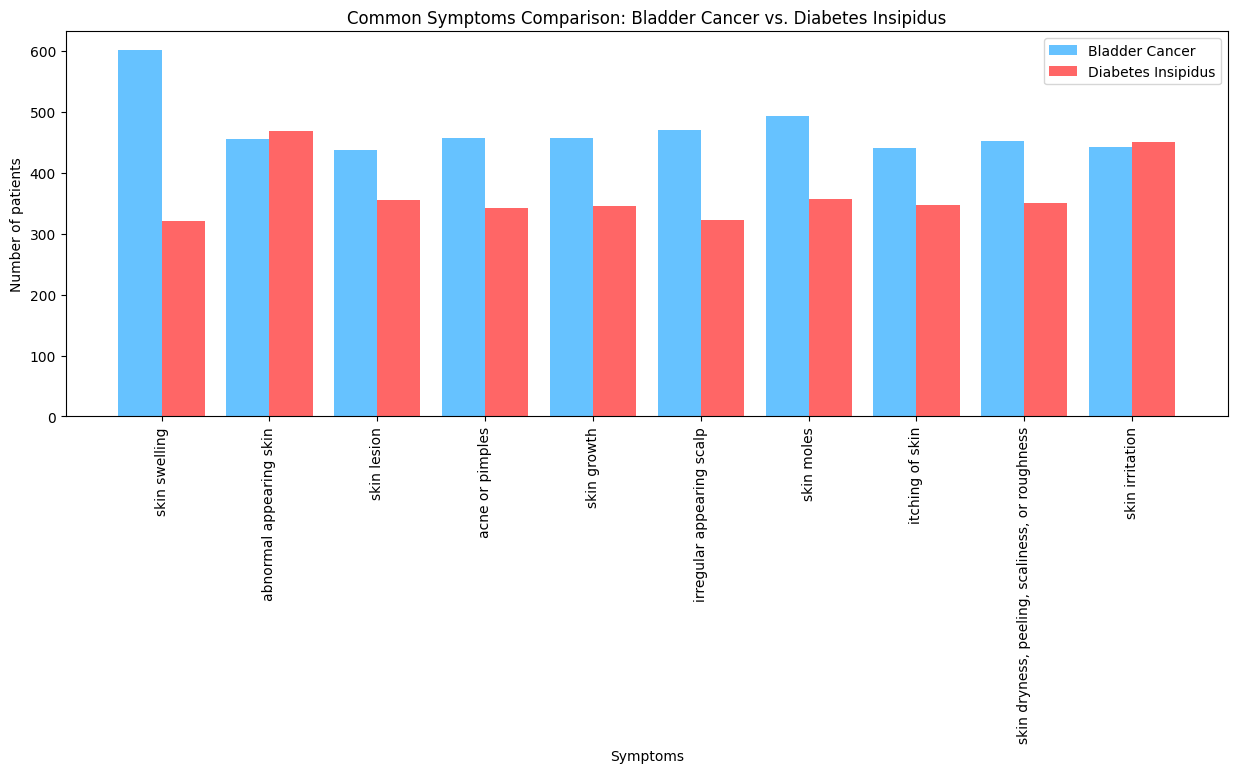
\includegraphics[width=\columnwidth]{cancer_diabet}
	\caption{number of samples of bladder cancer and diabets insipidus that have the same symptoms}\label{fig:cancer_diabet}
\end{figure}
\noindent

\begin{figure}[H]
	\centering
	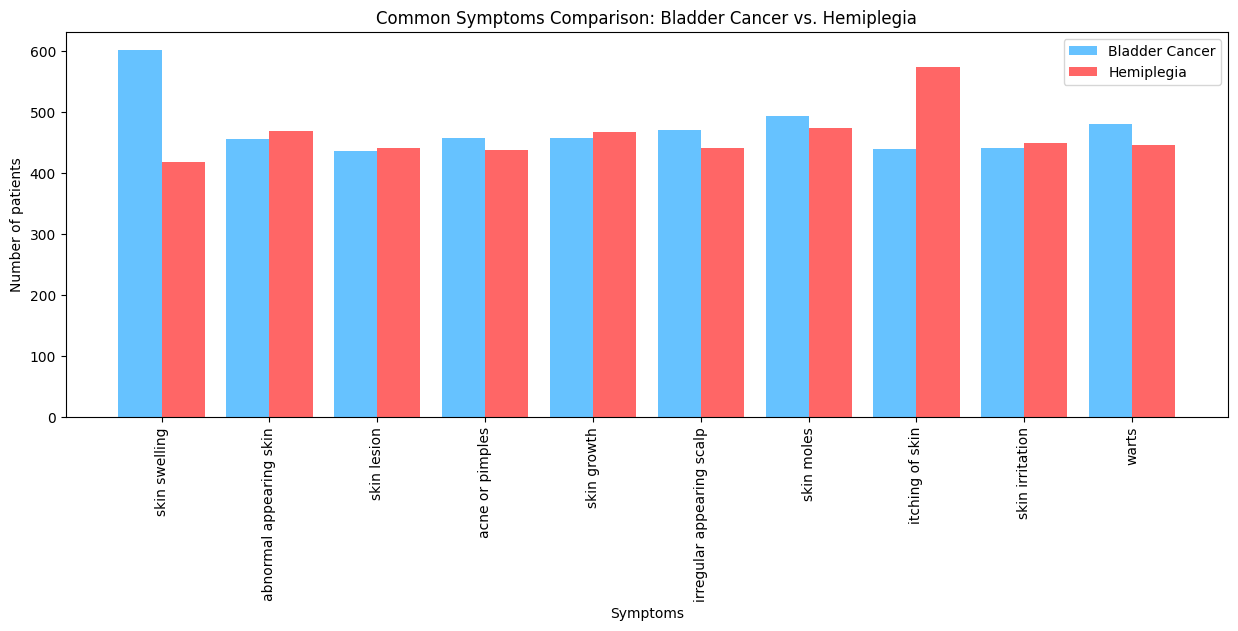
\includegraphics[width=\columnwidth]{cancer_hemiplegia.png}
	\caption{number of samples of bladder cancer and hemiplegia that have the same symptoms}\label{fig:caner_hemiplegia}
\end{figure}
\noindent

\subsubsection*{Analysis of otitis}

\begin{figure}[H]
	\centering
	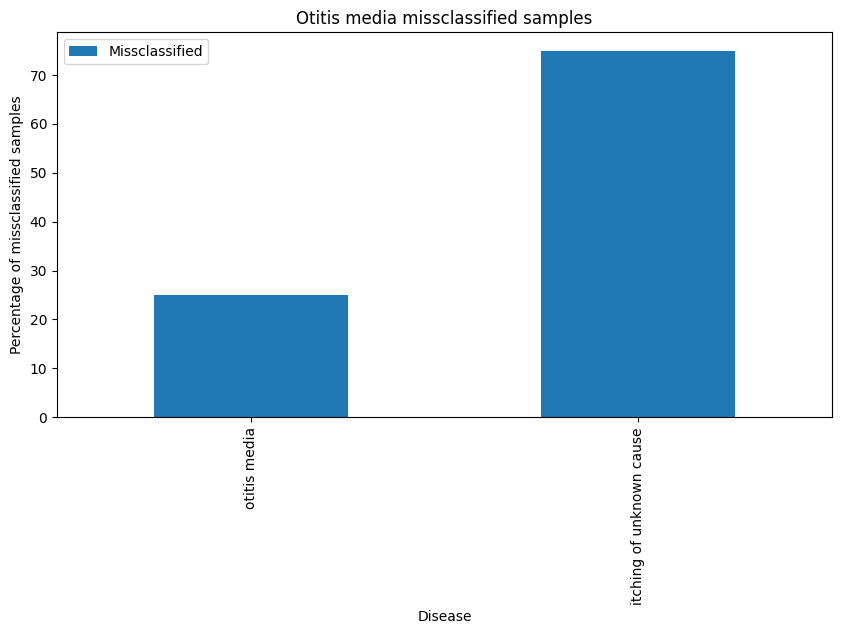
\includegraphics[width=\columnwidth]{otitis_missclassified.png}
	\caption{Percentage of otitis samples misclassified}\label{fig:otitis_missclassified}
\end{figure}
\noindent
\begin{figure}[H]
	\centering
	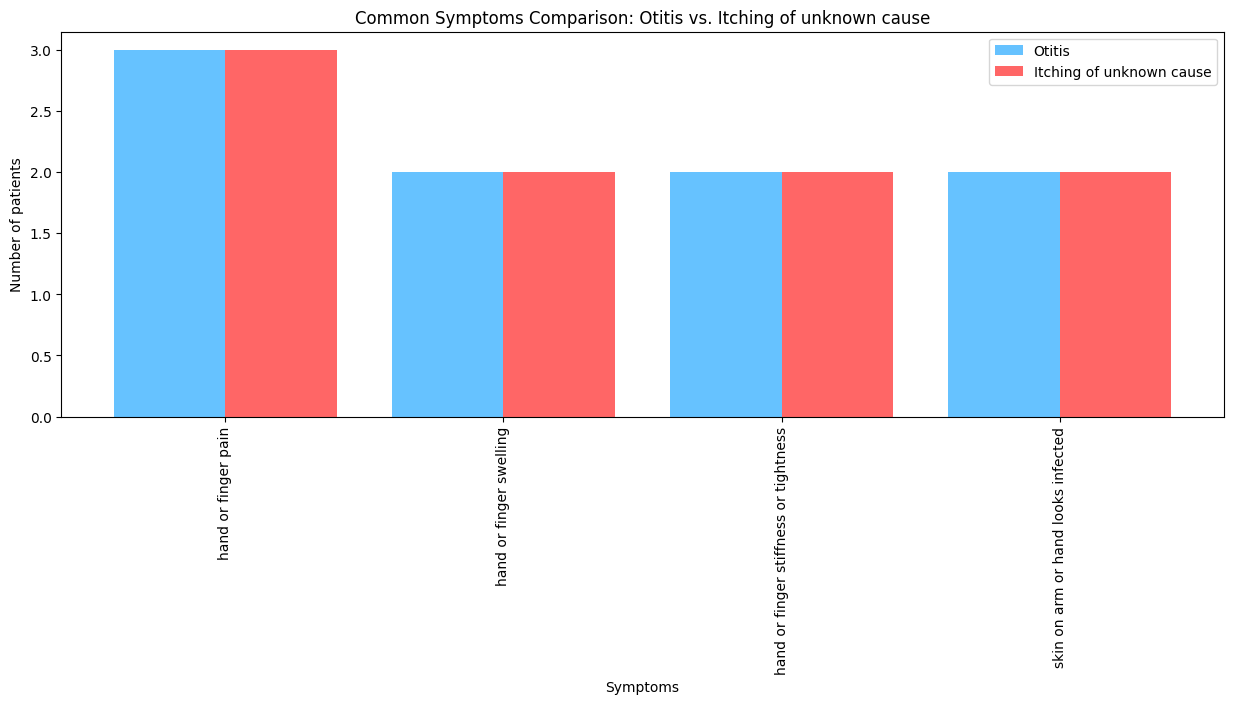
\includegraphics[width=\columnwidth]{otitis_itching.png}
	\caption{number of samples of otitis and itching of unknown cause that have the same symptoms}\label{fig:otitis_itching}
\end{figure}
\noindent

\subsection*{Most impactful symptoms}
\begin{figure}[H]
	\centering
	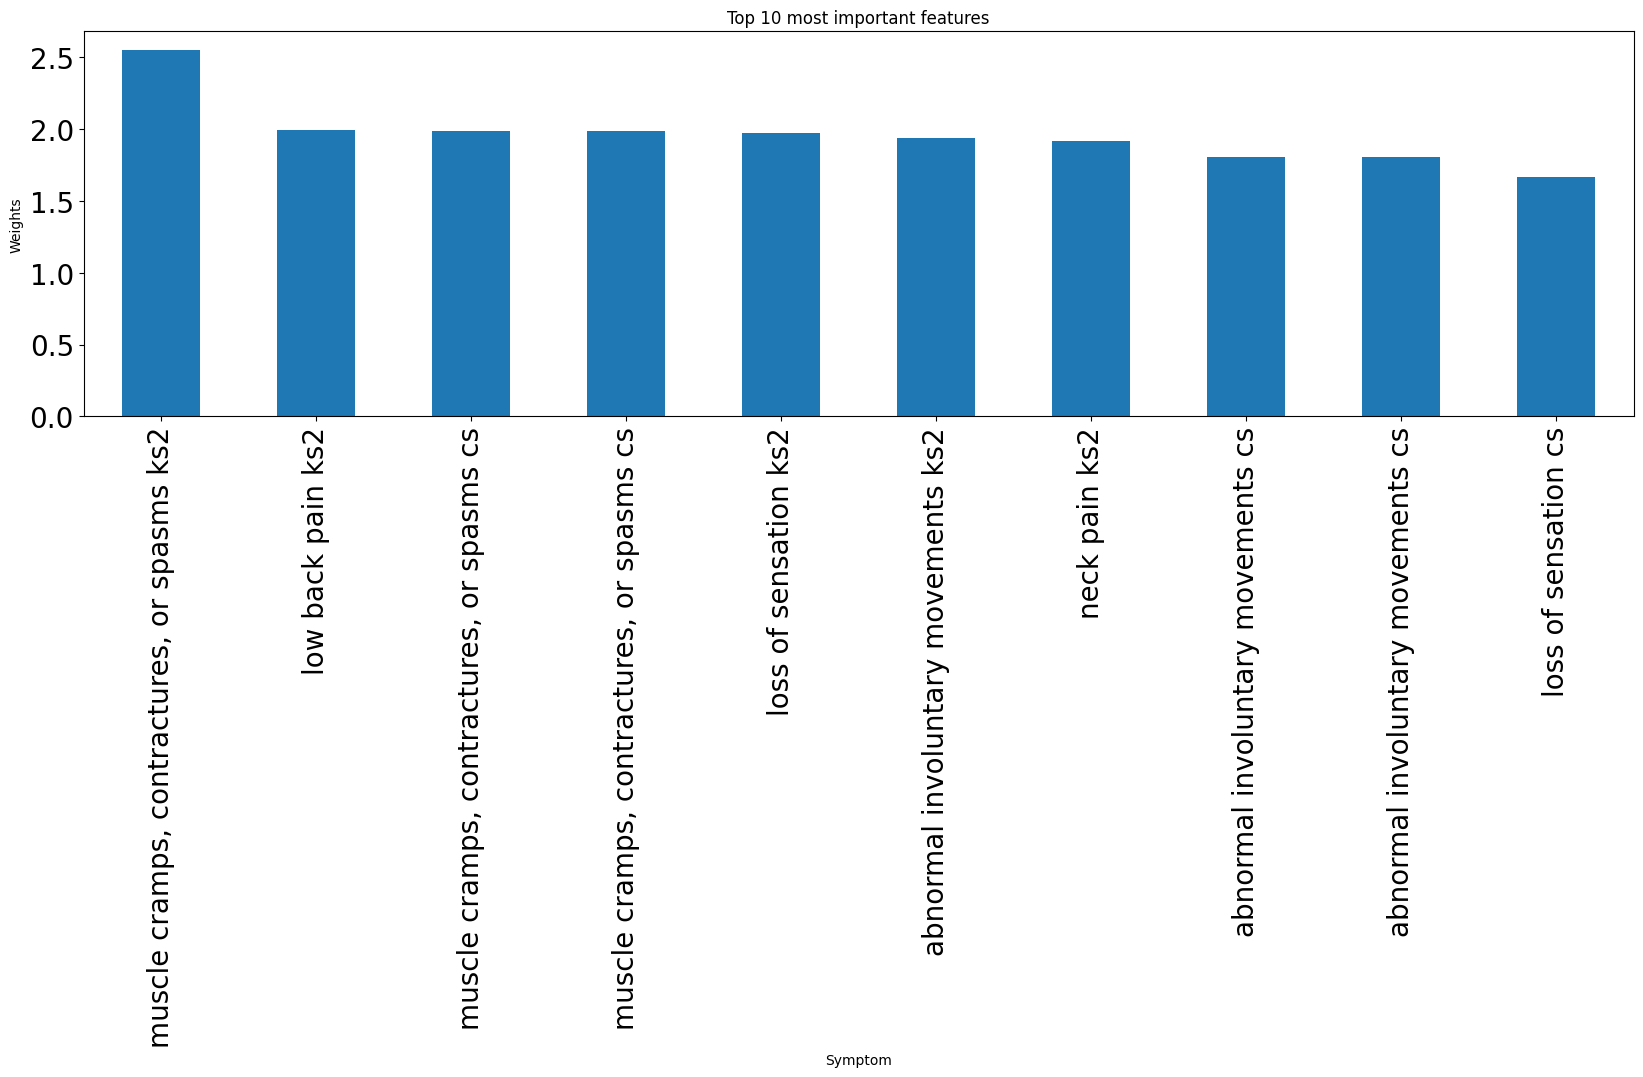
\includegraphics[width=\columnwidth]{most_important_features.png}
	\caption{10 most impactful features}\label{fig:most_important_features}
\end{figure}
\noindent

\subsection{Computational Complexity}
% MATTEO
% - apply the reduction technique based on symptoms importance (L1 and L2 combined in the 4 classes)
% - compare the performance of the reduced model with the original one
% - precision, recall, AUC, accuracy
% - compare the times needed to train the two models


% CRISTIAN
% - 6 Modelli: 3 con solo sintomi, 3 con nuove features
% - - Salvati (joblib) 
% - - Tempo di training


% - selected model performances (see which is the worst error or the most commonly misclassified diseases)
% - Compute accuracy and PR AUC
% - Compute the accuracy of the model dividing the data into the 4 classes (HighL1 - HighL2, LowL1 - HighL2, ...)
% - only with one hot symptoms (with optimal parameters both for one hot and other features) 
% - with new features 
% - reduction in computational complexity

% ---------------------- Conclusion -----------------------------

\section{Conclusion}

Our study successfully integrates network analysis with machine learning to enhance disease prediction models in healthcare.
By analyzing symptom-disease networks using Symptom Influence (SI) and Disease Influence (DI) indices, we uncovered
critical patterns essential for accurate disease prediction. These indices revealed diverse symptom-disease associations,
guiding the selection of features for our models.\\
Logistic Regression emerged as the most effective model, balancing accuracy and complexity, particularly when augmented with network-based features.
This model demonstrated high accuracy and managed to capture complex patterns without significant overfitting.\\
A key achievement of our study is the effective balance between feature reduction and model performance.
Focusing on significant symptoms, we reduced training time substantially while maintaining high accuracy.
This approach is especially valuable in real-world applications where computational efficiency is crucial.\\
The study, however, also recognized challenges in disease prediction, as highlighted by the analysis of specific
diseases like bladder cancer and otitis media. These cases illustrated the intricacies involved in disease classification
and the necessity for continuous model refinement.
\section{Limits and Future Works}
\label{sec:future_works}

In the pursuit of our final model, we navigated through a series of pivotal decisions, ranging from model selection, feature choices, 
and the intricate interplay of normalization techniques to hyperparameter tuning. These decisions, while steering us toward a robust model, 
come with inherent trade-offs, potentially leading to suboptimal outcomes. Here, we discuss some limitations in our approach and suggest 
avenues for future exploration.

\subsection{Limits}
\label{subsec:limits}

\begin{itemize}
\item \textbf{Feature Selection}: The selection of optimal features, as depicted in Figure \ref{fig:ML_operative_flow}, occurred 
before hyperparameter tuning. This sequential approach may result in the choice of an ostensibly optimal feature set, 
as both aspects are tightly linked.

\item \textbf{Hyperparameter Tuning}: The determination of the best hyperparameter combination relied on accuracy as 
the sole metric. While we employed a stratified cross-validation on a balanced dataset for a reliable accuracy estimate, 
a more comprehensive approach should encompass additional metrics such as precision, recall, and F1-score.

\item \textbf{Feature Reduction}: The feature reduction process evenly separated the four classes of symptoms and commenced 
retaining features from the class demonstrating the highest predictive power. This approach may yield suboptimal results, as a 
specific threshold might exist beyond which the predictive power of a feature diminishes. 
To better clarify this concept, let's consider the following example: suppose we have only two classes of symptoms, evenly distributed 
using the median as a threshold on the degree value. Suppose also that the predictive power of the features is the same for both classes.
In this case we cannot actually say that the degree doesn't impact the predictive power of the model. Indeed in the high degree class
we can have put lots of features with a degree not sufficiently high to become less relevant and these diseases end up
altering the result of the whole class, especially in a power law distribution context. 
A refined strategy involves employing a manual threshold for the degree value, identifying truly impactful features, 
potentially resulting in unbalanced classes.

\end{itemize}

\subsection{Future Work}

\begin{itemize}
\item \textbf{Symptoms Communities}: The features extracted from symptom communities were integrated into the model based on their 
inherent ability to capture relevant information. A potential enhancement involves leveraging this knowledge explicitly, using it as prior 
probability for the model. This entails favoring the most common diseases associated with the patient's symptoms and their communities.

\item \textbf{Multi-label Classification}: Our current approach treats diseases as independent entities. However, some diseases 
may be intricately connected. A prospective improvement entails treating diseases as a multi-label classification problem. 
For instance, the model could output the three most likely diseases instead of a singular one.

\item \textbf{Disease Complexity Analysis}: Our accuracy analysis extends to different classes of diseases based on their L1 and L2 values. 
A potential refinement involves a nuanced exploration of disease complexity, adjusting L1 and L2 thresholds to maximize accuracy 
differentials among disease classes. This approach would facilitate an in-depth analysis of diseases that pose higher prediction challenges.


\end{itemize}

% - our approach in feature selection and parameters search is not optimal 
% - list the possible issues (e.g. we are training model on diverse features with the optimal parameters for other features)
% - exploit the knowledge of symptoms communities and their most pointed diseases, using it at prior probability for the model classification


\section{Appendix}

% ------------- Appendix Figures -------------
% Figures to be placed in the appendix

\begin{figure}[H]
	\centering
	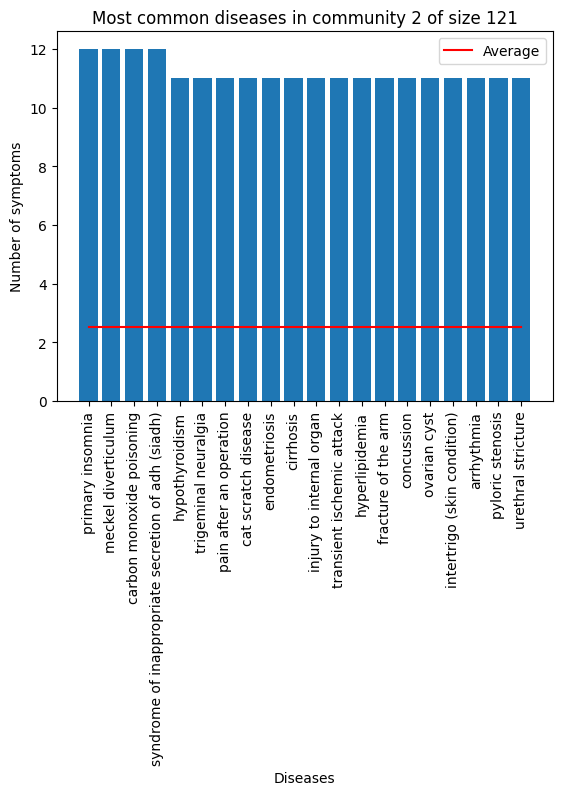
\includegraphics[width=\columnwidth]{com2_symptoms.png}
	\caption{Community 2 of symptoms}
	\label{fig:com2_symptoms}
 \end{figure}
 \noindent
 \begin{figure}[H]
	\centering
	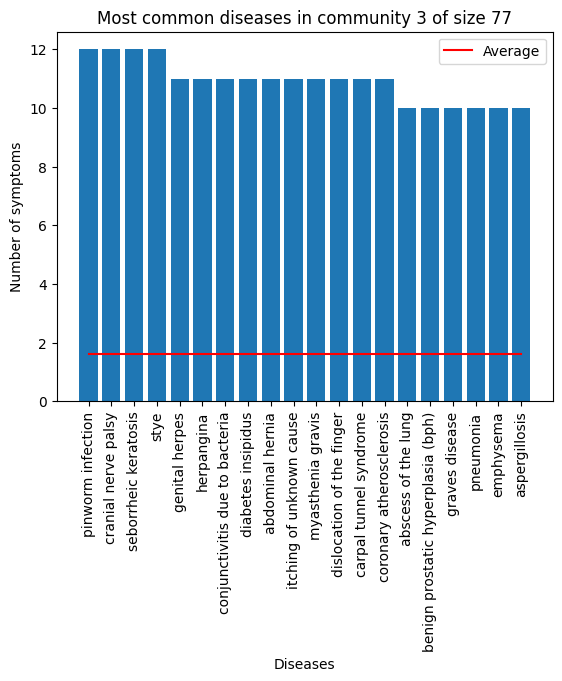
\includegraphics[width=\columnwidth]{com3_symptoms.png}
	\caption{Community 3 of symptoms}
	\label{fig:com3_symptoms}
 \end{figure}
 \noindent
 
 
 \begin{figure}[H]
	\centering
	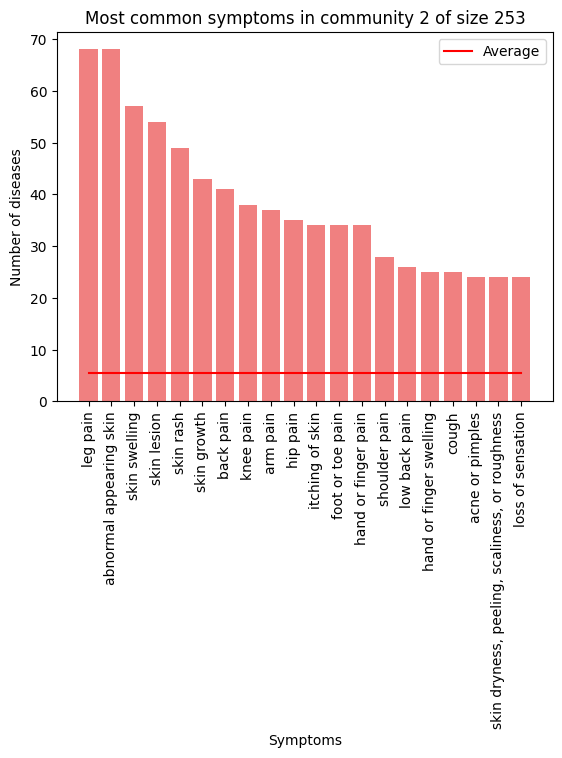
\includegraphics[width=\columnwidth]{com2_diseases.png}
	\caption{Community 2 of diseases}
	\label{fig:com2_diseases}
 \end{figure}
 \noindent
 \begin{figure}[H]
	\centering
	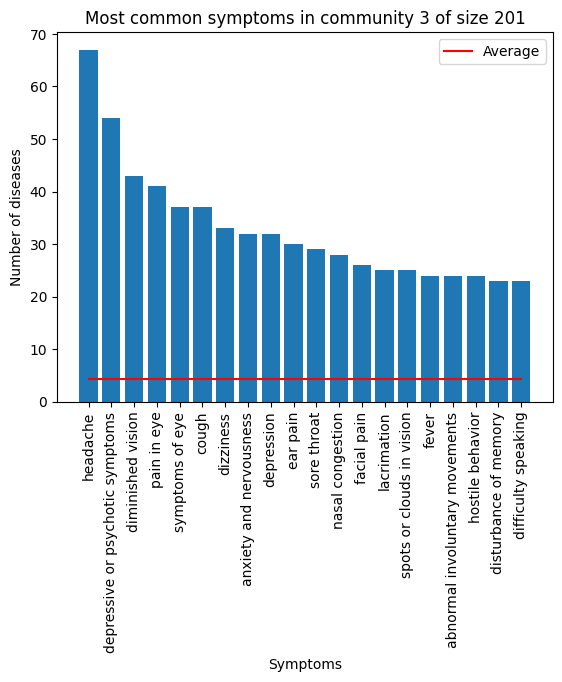
\includegraphics[width=\columnwidth]{com3_diseases.png}
	\caption{Community 3 of diseases}
	\label{fig:com3_diseases}
 \end{figure}
 \noindent

\clearpage
\printbibliography

\end{document}